\section{Experiments and Results}

\subsection{Performance Evaluation}
\subsubsection{Kosarak PFP 100\textbar 1000\textbar 500 partitions}
~\autoref{fig:kosarak_pfp_001} presents PFP with different partitions sizes. Best performance achieved for 500 partitions.

\subsubsection{PFP}
We first evaluate the performance of PFP to better understand its behaviour. ~\autoref{fig:kosarak_pfp_001} presents PFP performance on the ~\autoref{data:kosarak} with different partitions sizes. Best performance achieved for 500 partitions. For ~\autoref{data:10Msynt} ~\autoref{fig:T15I5D10000N100_pfp_0001}, best performance is achieved for 1000 partitions. And ~\autoref{fig:T15I5D1000N10_pfp_00001} for ~\autoref{data:1Msynt} with support of 0.00001 (more than 10 items are frequent). 100 and 500 have the better performance.

For tree size, 
%\begin{figure}
%  \centering
%  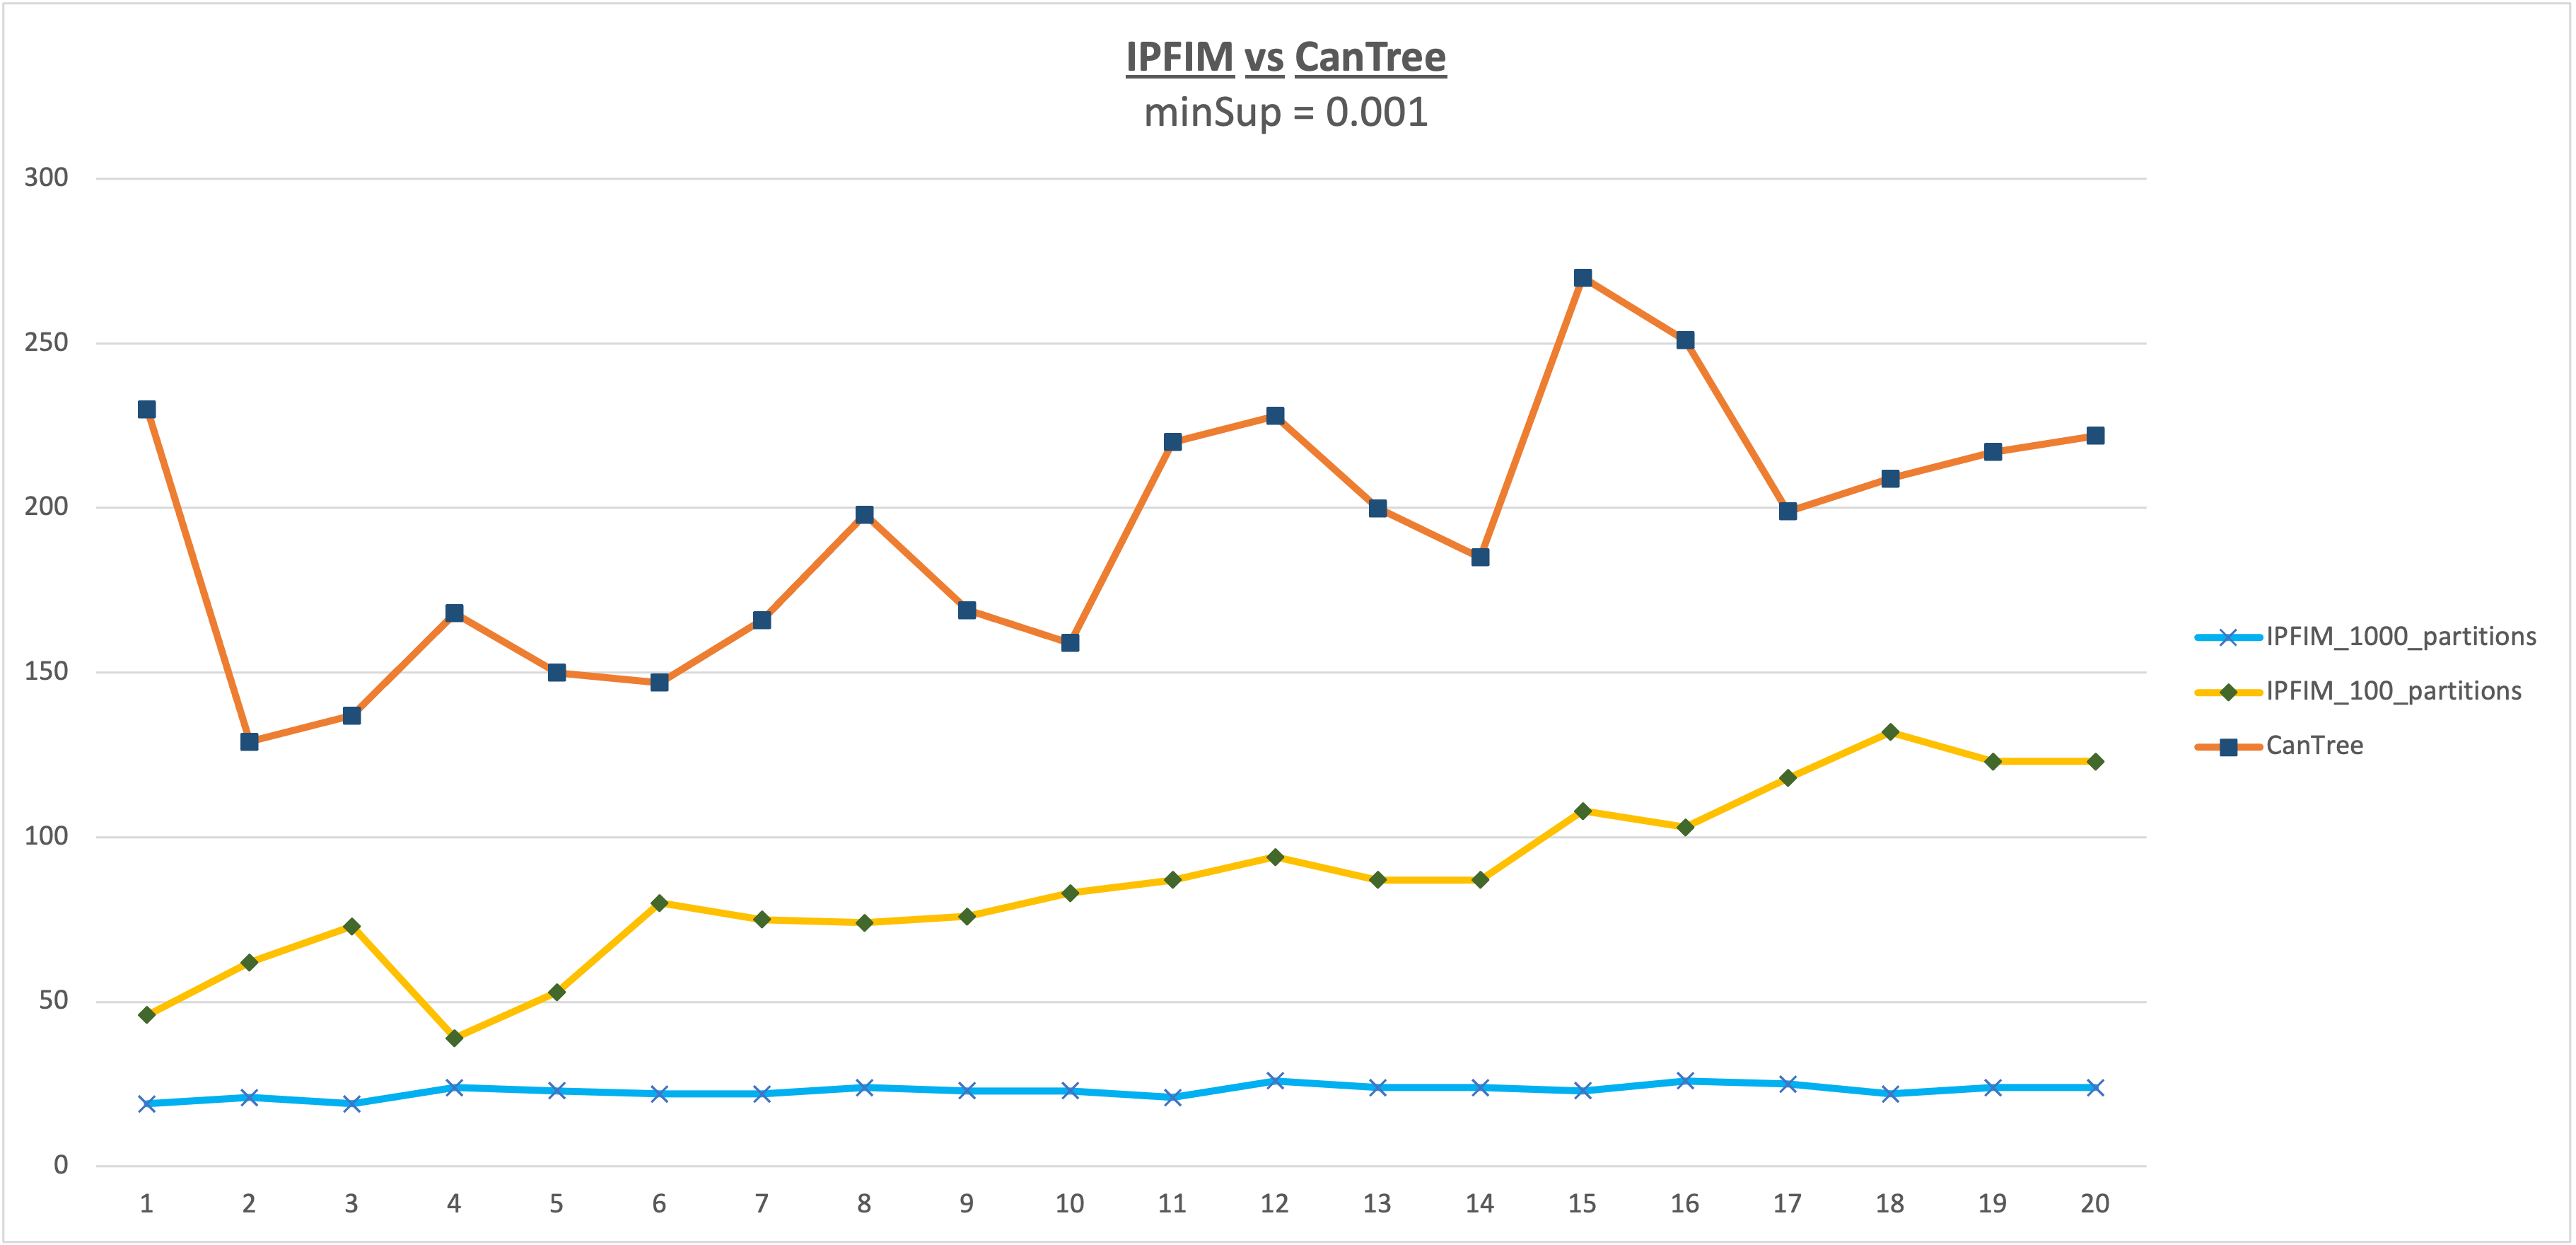
\includegraphics[width=\linewidth]{figures/IPFIM_VS_CANTREE_001_T15D1M10K}
%  \caption{IPFIM vs CanTree T15D1M10K}
%  \label{fig:IPFP1M0001}
%\end{figure}

\begin{figure}
  \centering
  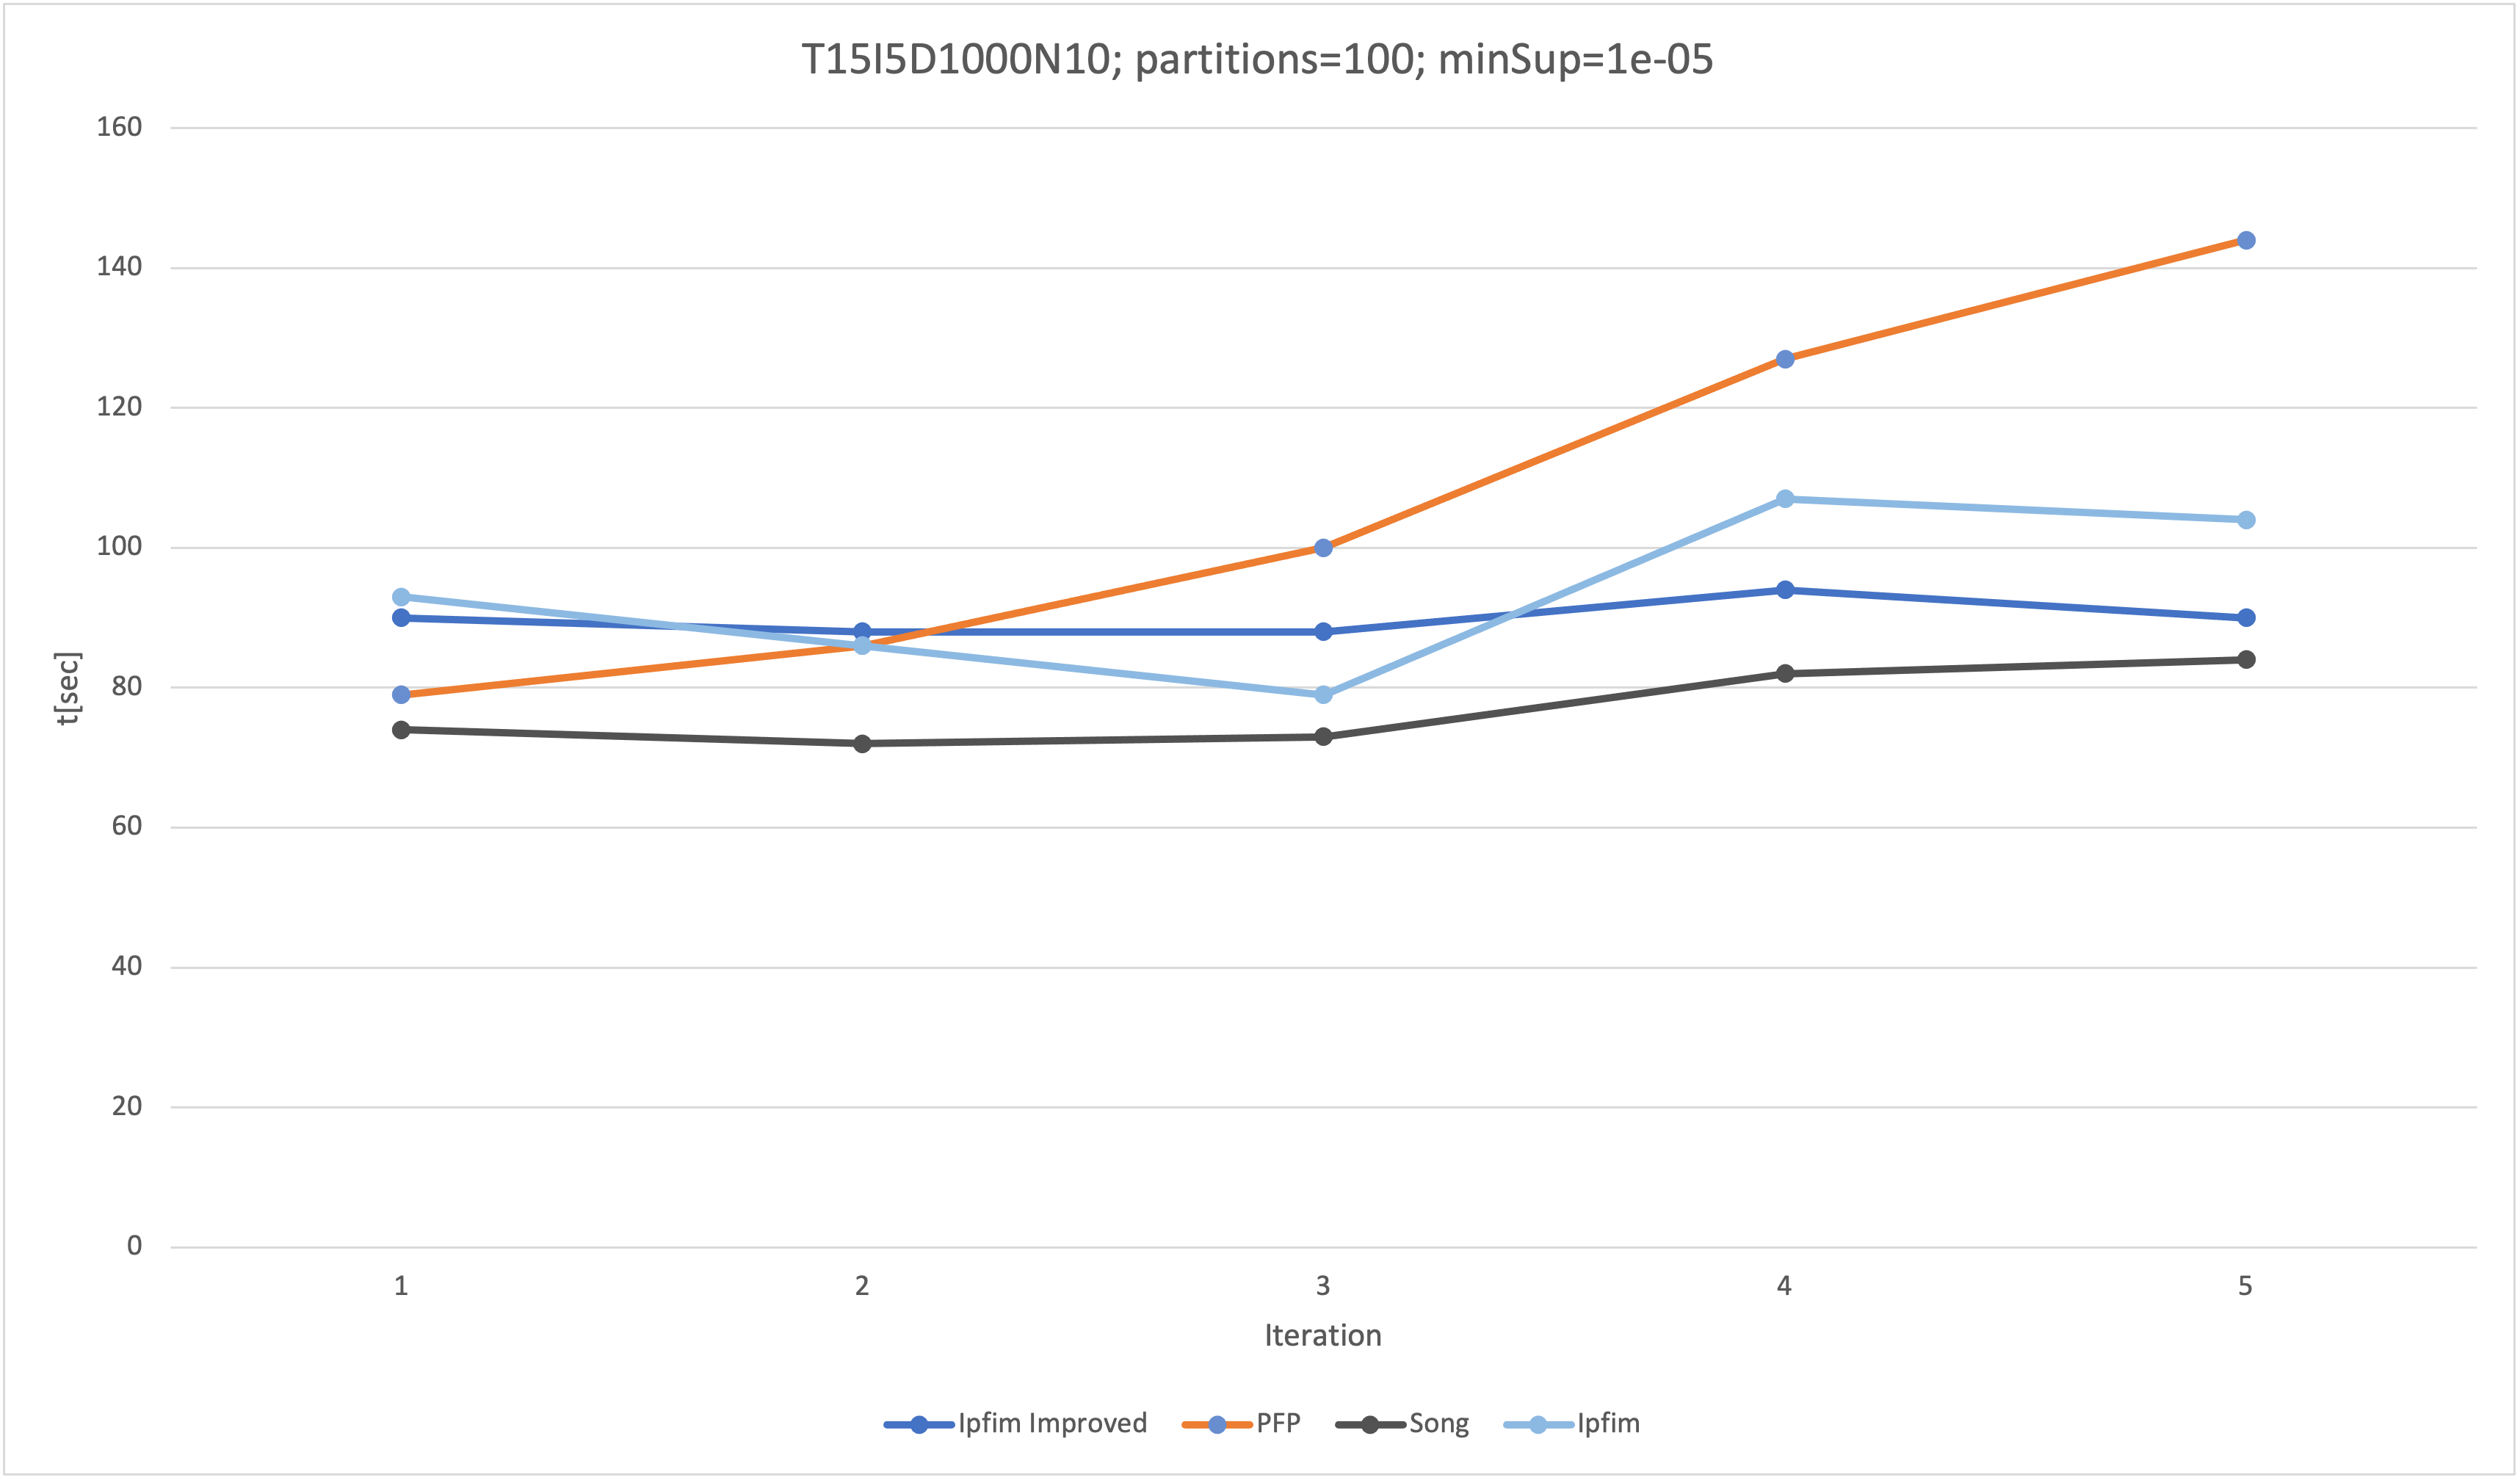
\includegraphics[width=\linewidth]{figures/4iterations/T15I5D1000N10_100_0005}
  \caption{T15I5D1000N10 100 partitions}
  \label{fig:T15I5D1000N10_100_0005}
\end{figure}

\begin{figure}
  \centering
  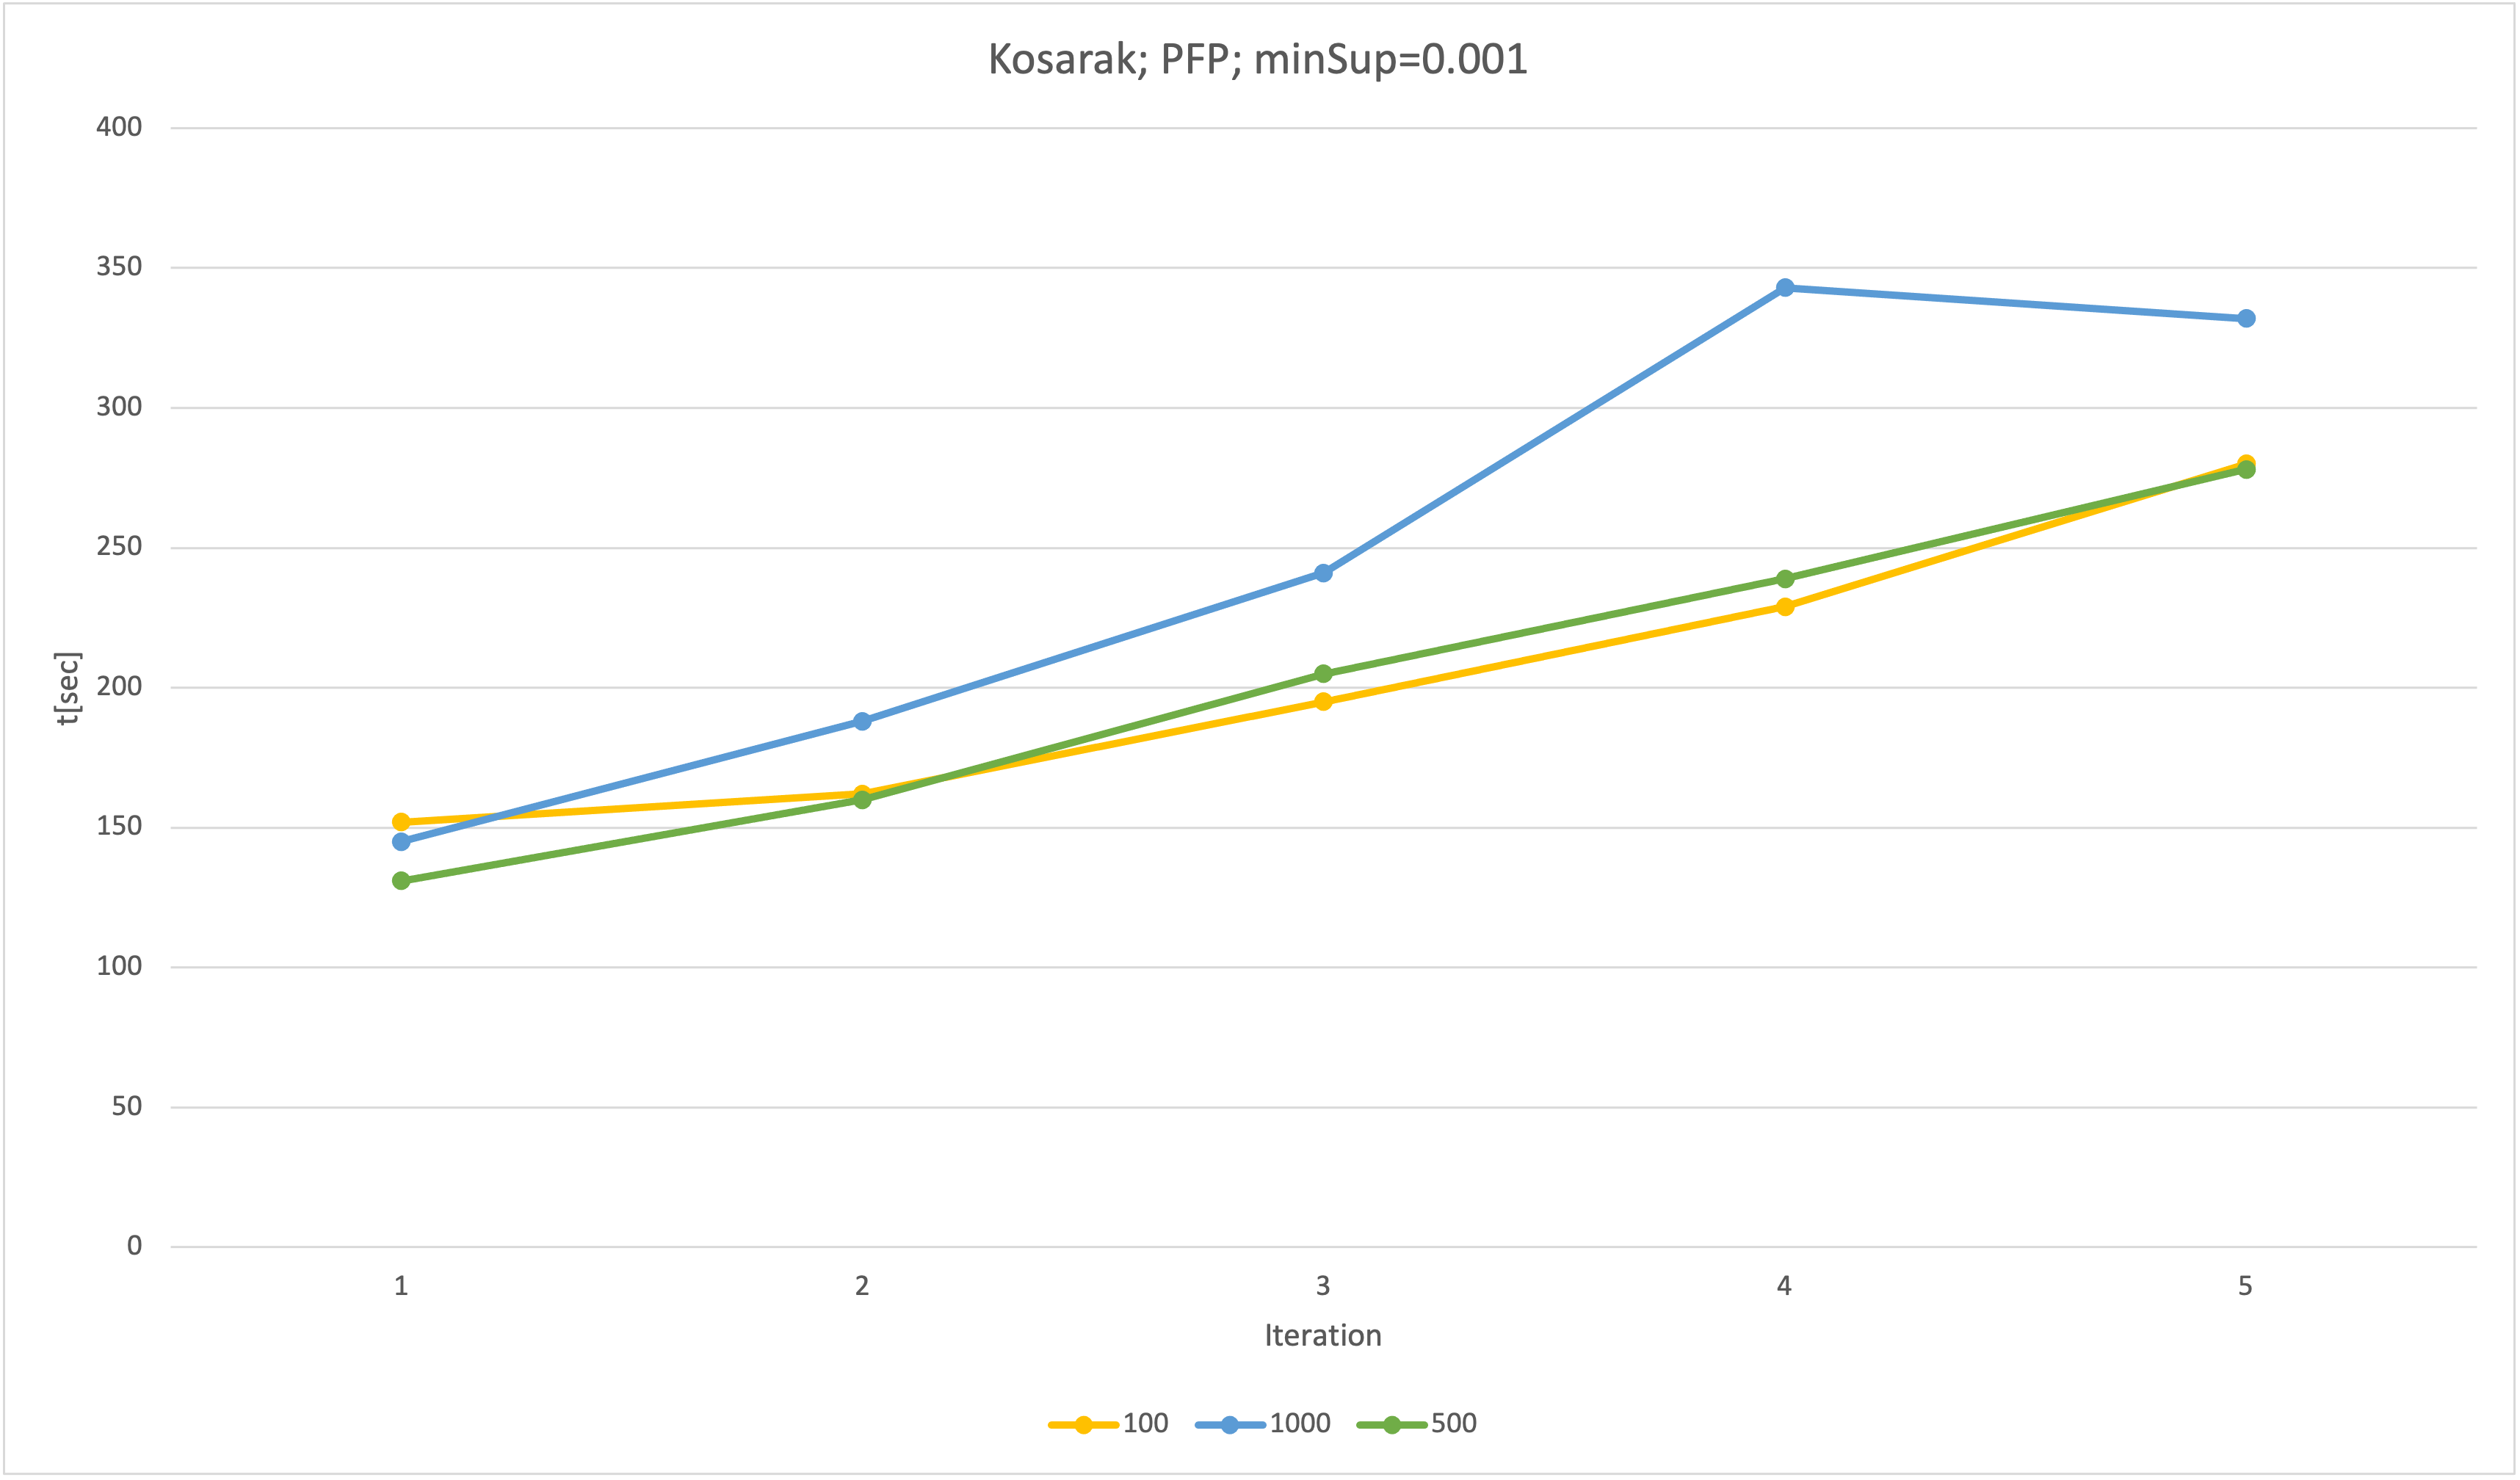
\includegraphics[width=\linewidth]{figures/4iterations/kosarak_pfp_001}
  \caption{kosarak, minSup = 0.001, PFP 100|1000|500 partitions}
  \label{fig:kosarak_pfp_001}
\end{figure}

\begin{figure}
  \centering
  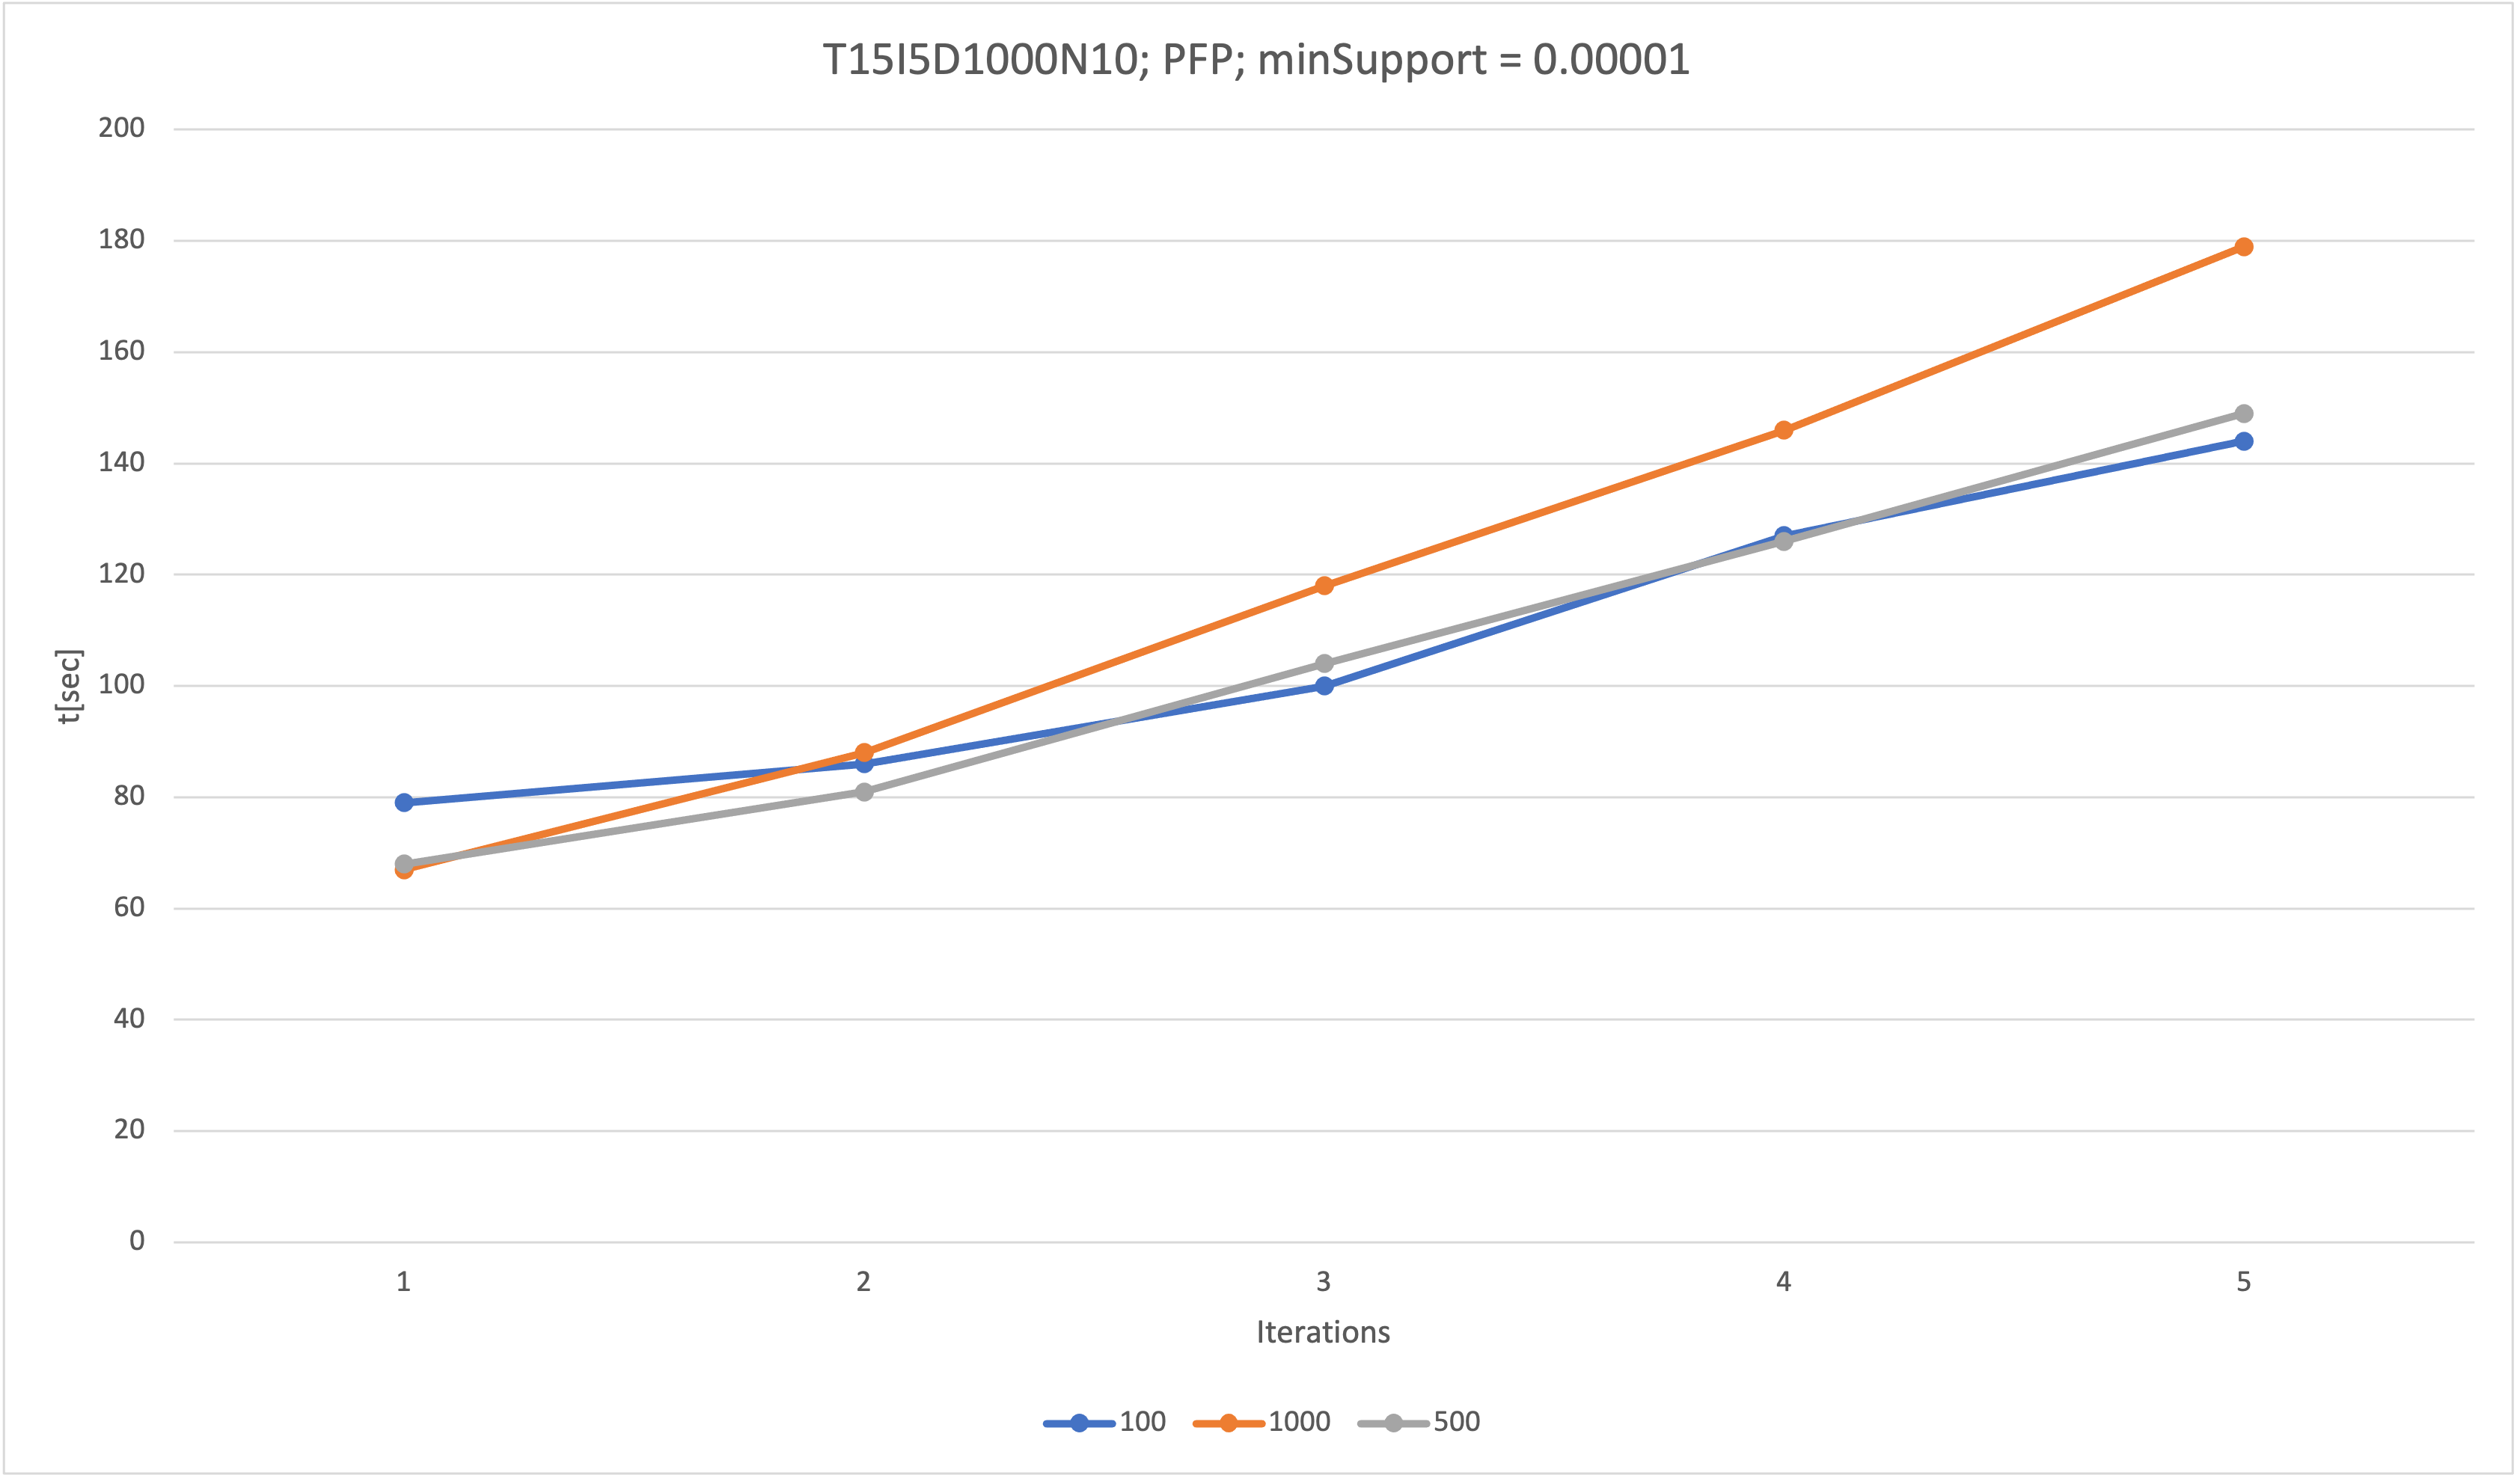
\includegraphics[width=\linewidth]{figures/4iterations/T15I5D1000N10_pfp_00001}
  \caption{T15I5D1000N10, minSup = 0.00001, PFP 100|1000|500 partitions}
  \label{fig:T15I5D1000N10_pfp_00001}
\end{figure}

\begin{figure}
  \centering
  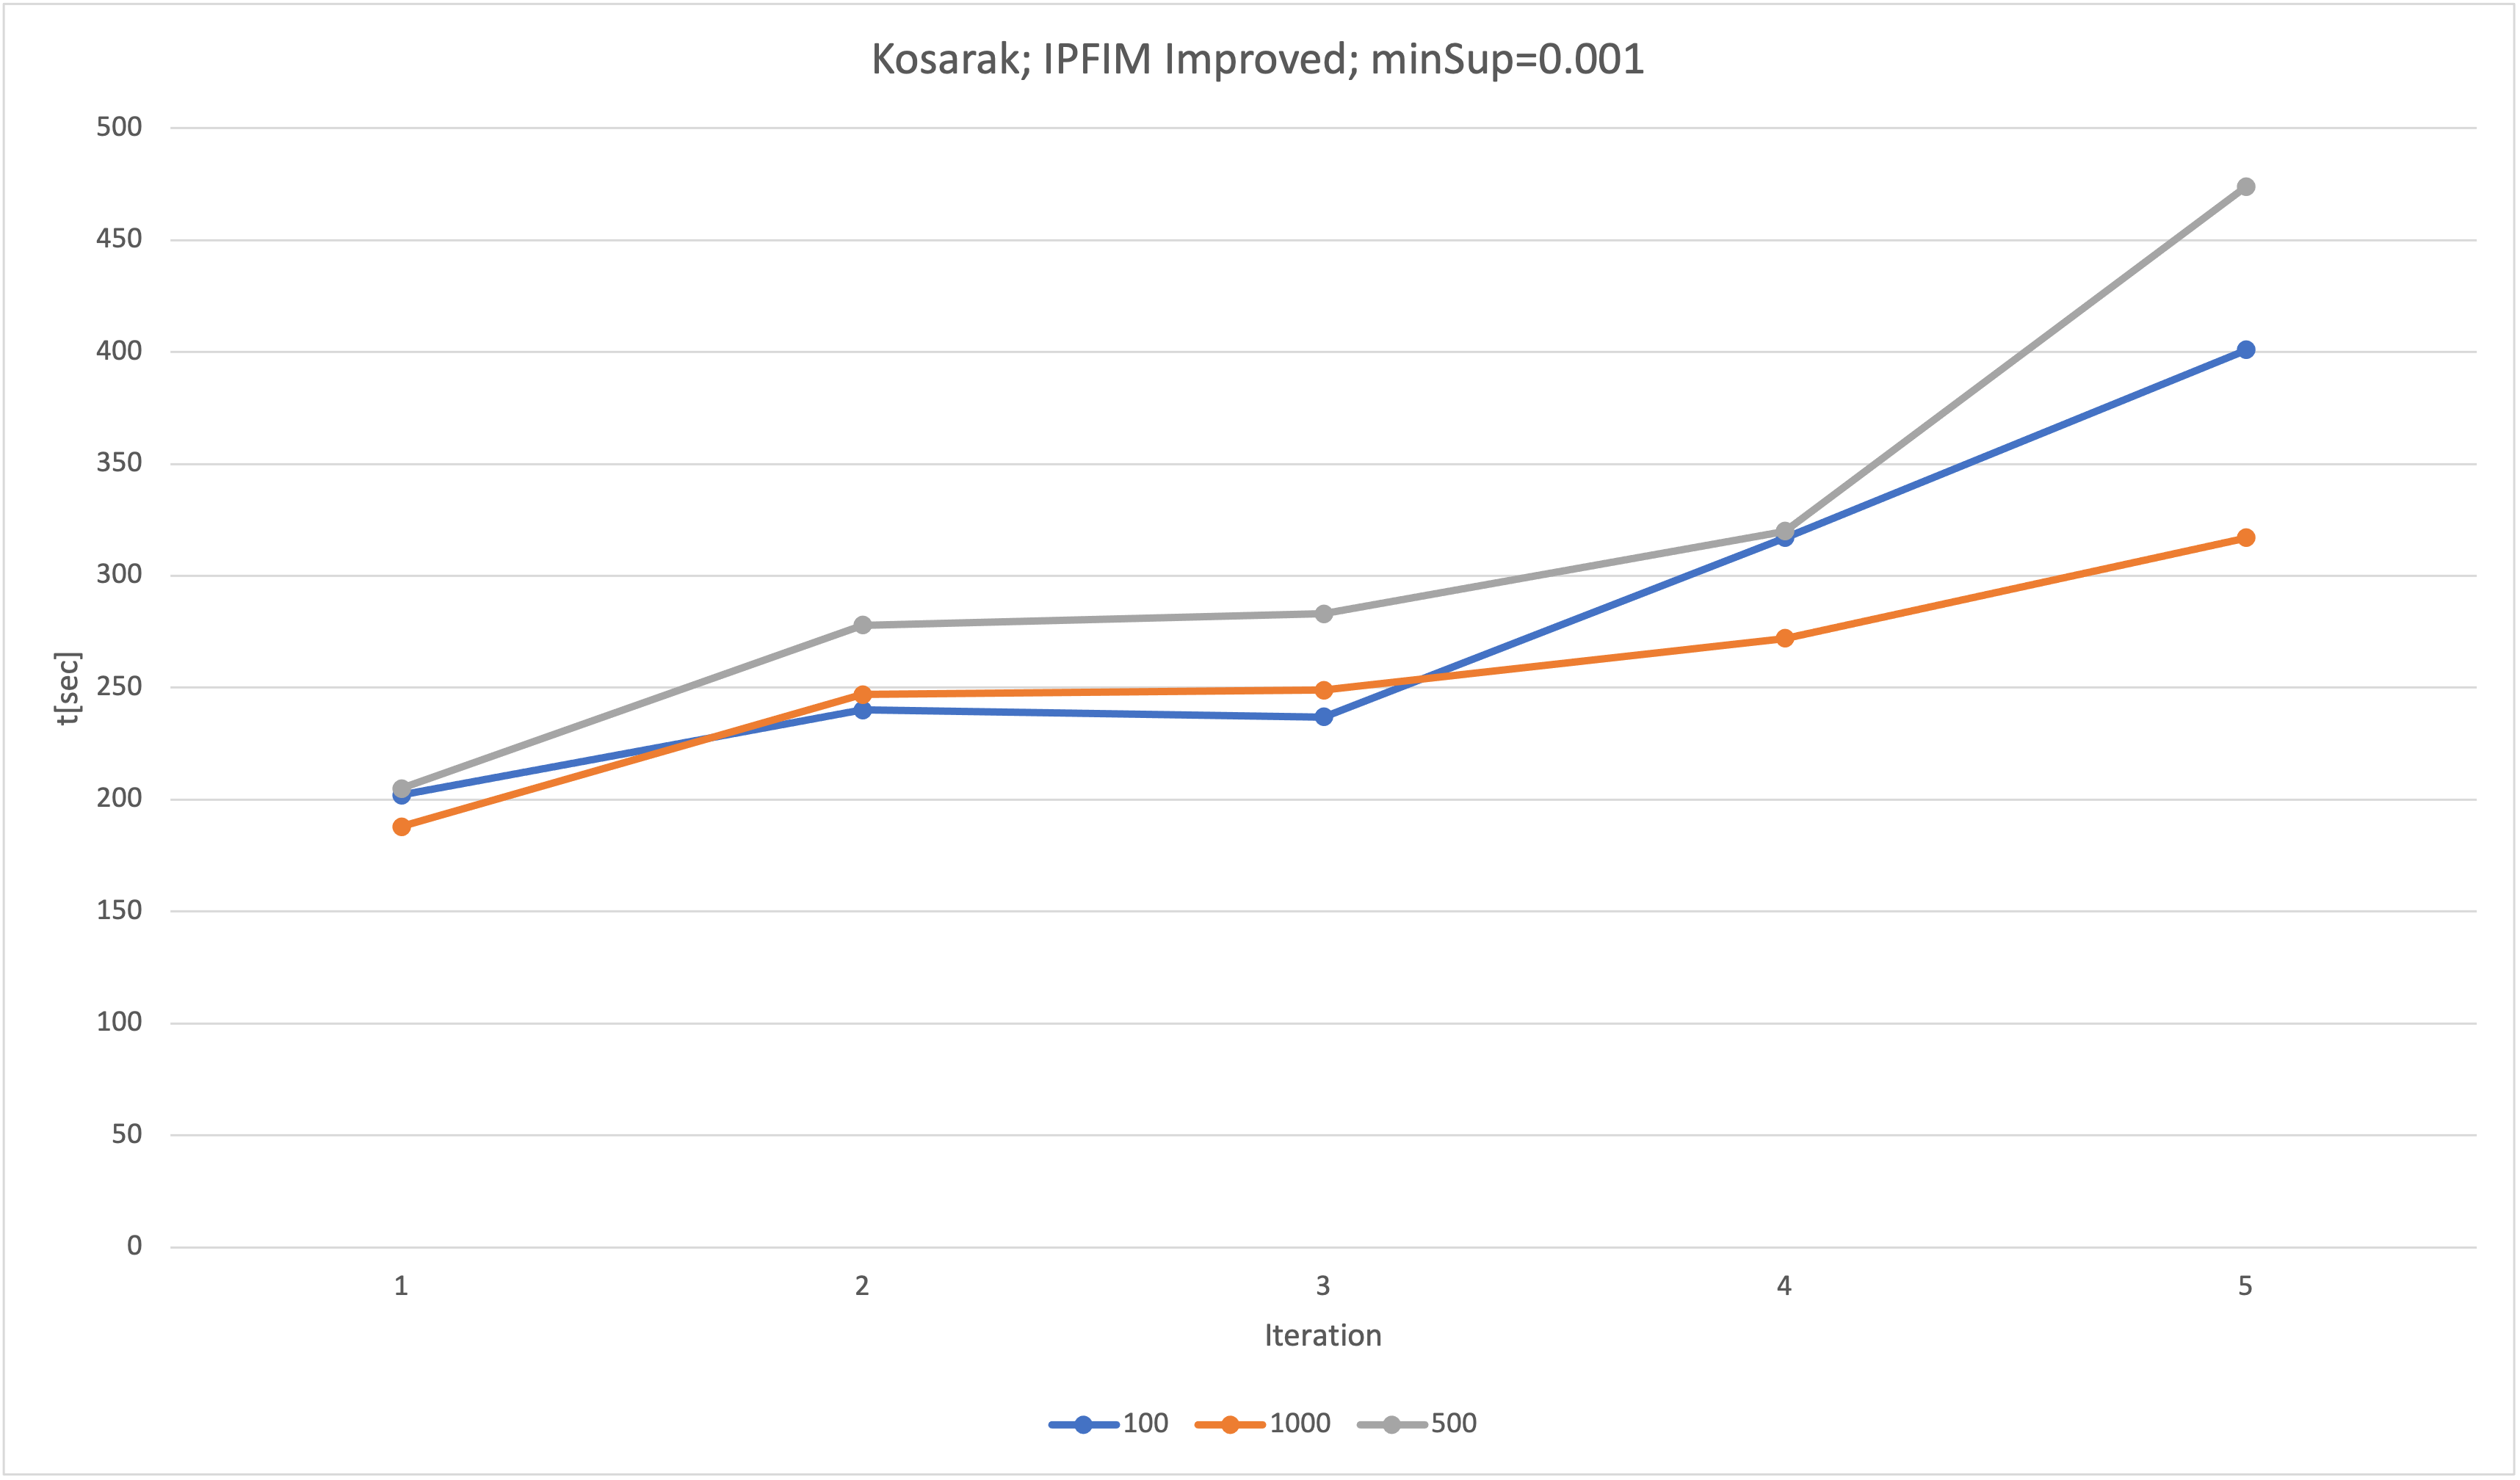
\includegraphics[width=\linewidth]{figures/4iterations/kosarak_ipfim_imp_001}
  \caption{kosarak, minSup = 0.001, IPFIM Improved 100|1000|500 partitions}
  \label{fig:kosarak_ipfim_imp_001}
\end{figure}

\begin{figure}
  \centering
  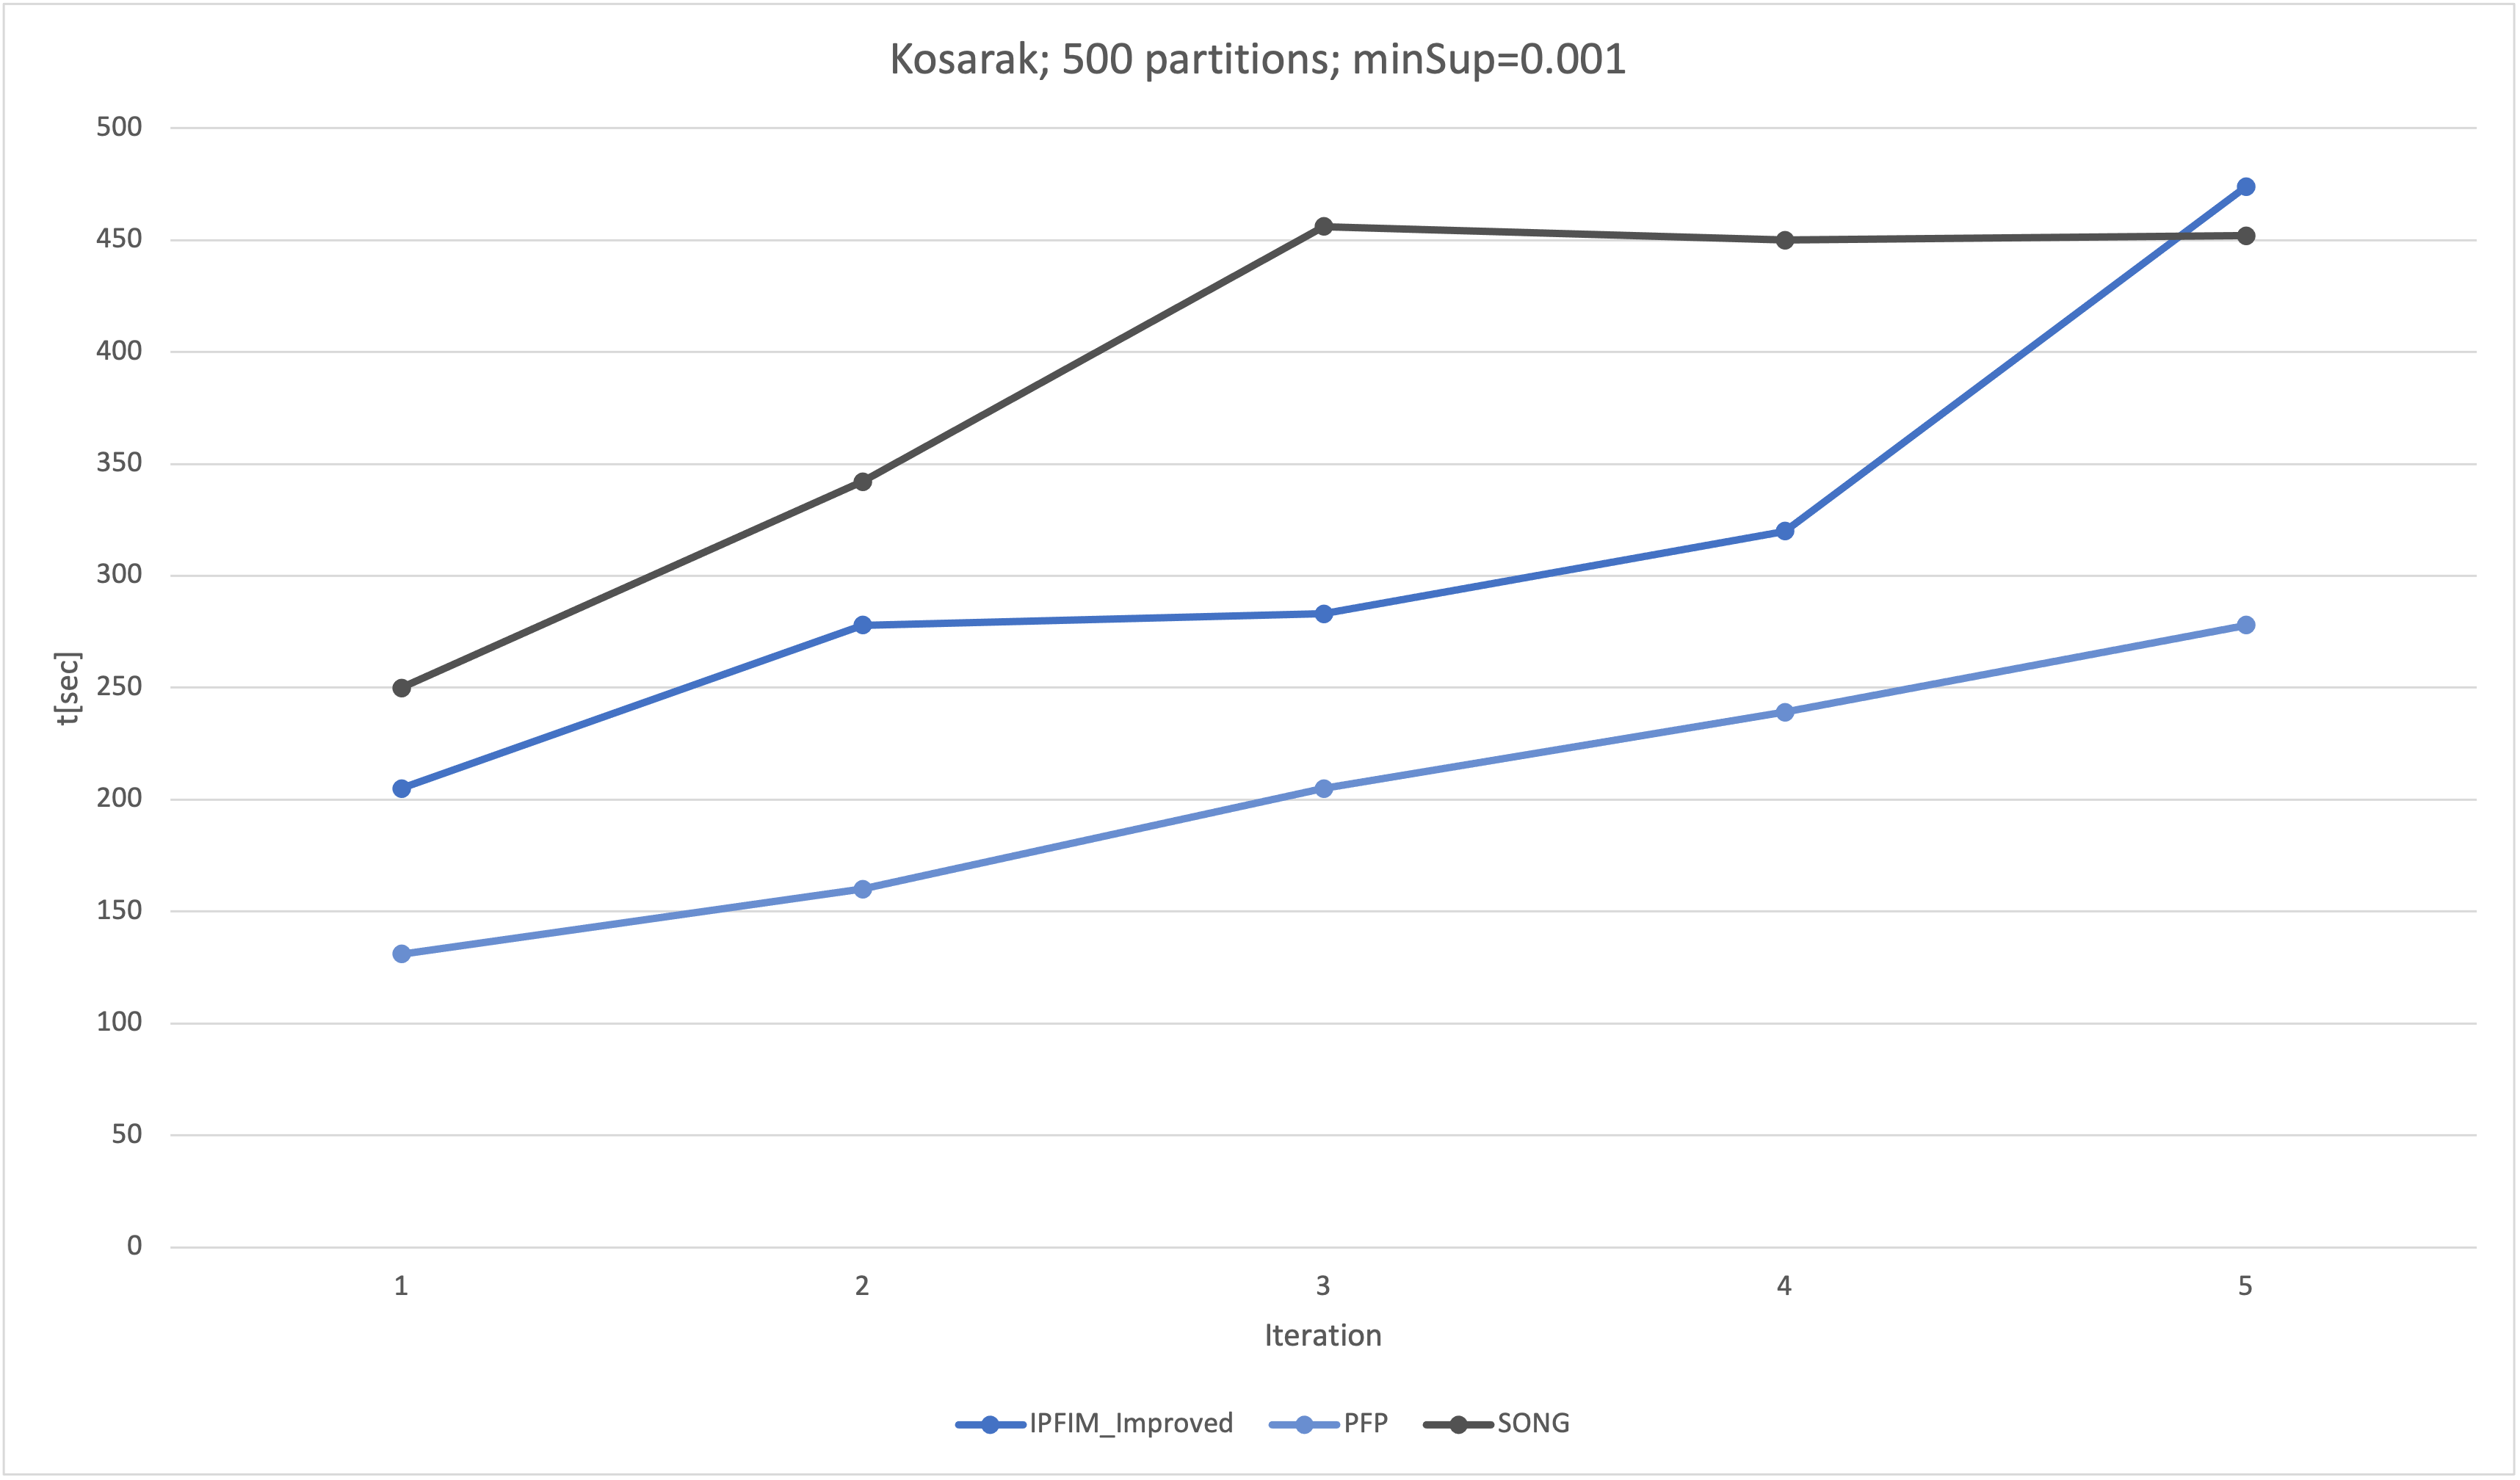
\includegraphics[width=\linewidth]{figures/4iterations/kosarak_500part_001}
  \caption{kosarak, minSup = 0.001,  partitions = 500}
  \label{fig:kosarak_500part_001}
\end{figure}

\begin{figure}
  \centering
  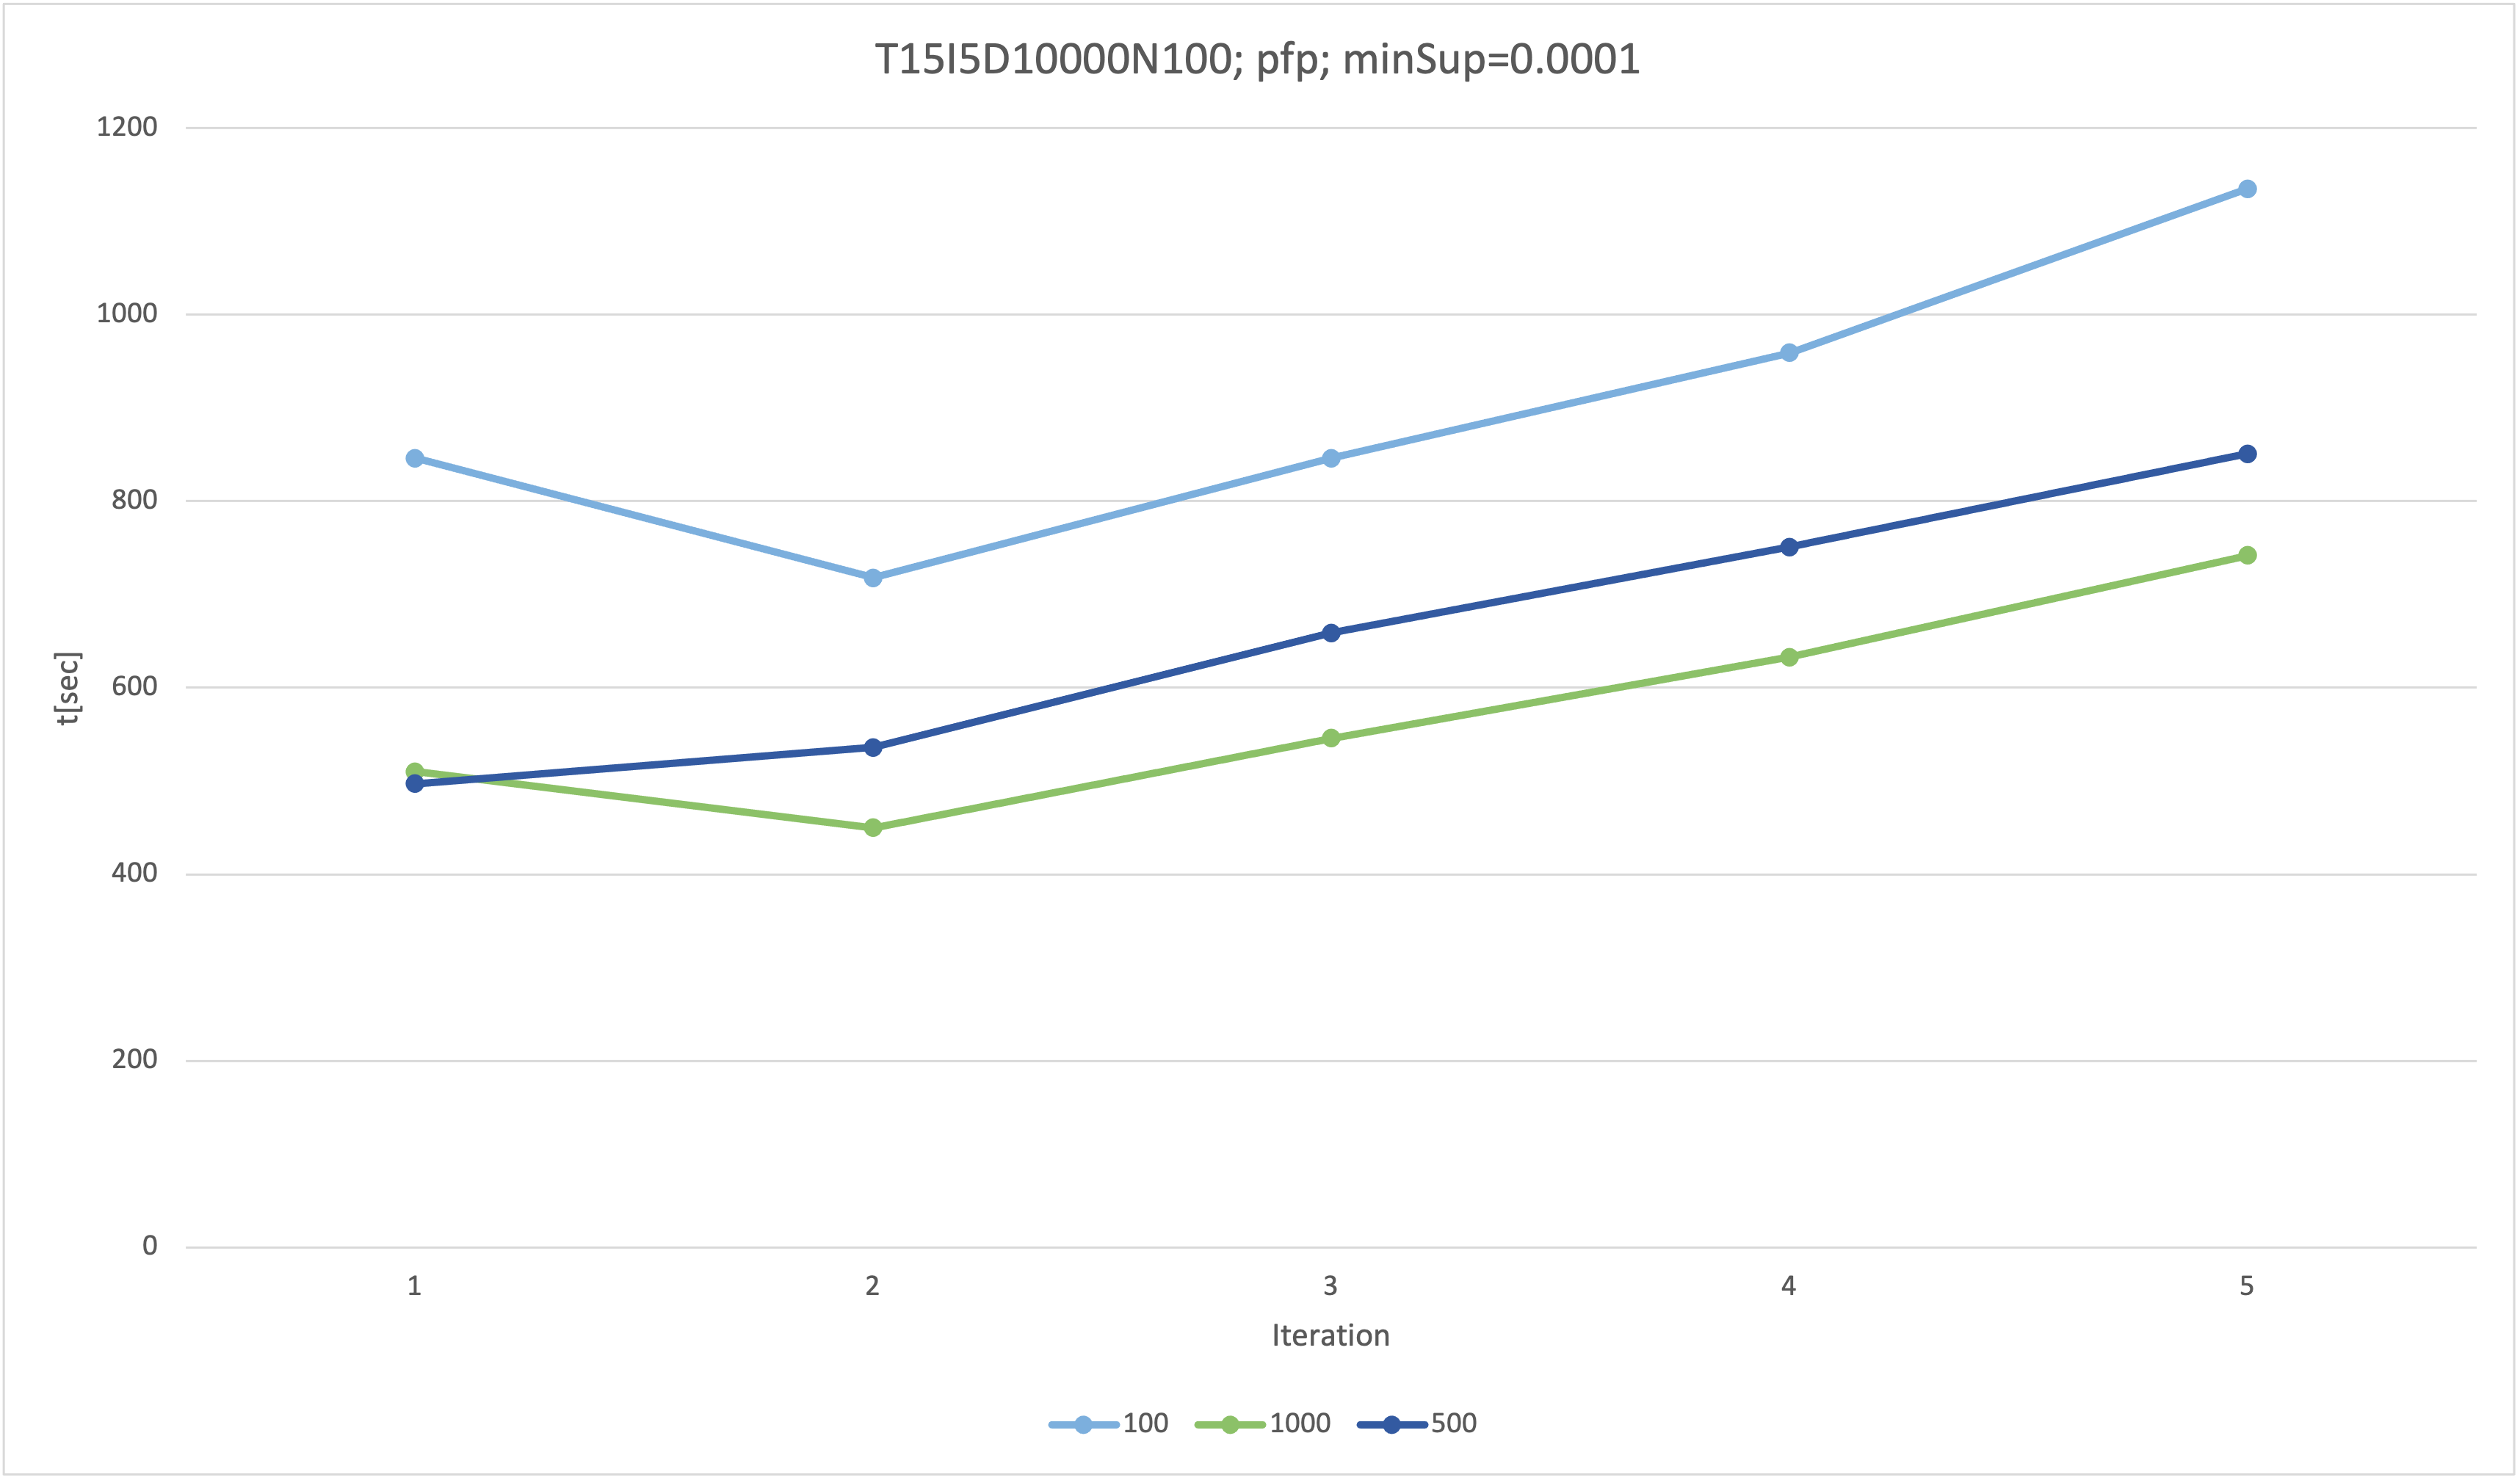
\includegraphics[width=\linewidth]{figures/4iterations/T15I5D10000N100_pfp_0001}
  \caption{T15I5D10000N100, minSup = 0.0001,  PFP 100\textbar 1000\textbar 500 partitions}
  \label{fig:T15I5D10000N100_pfp_0001}
\end{figure}


\begin{figure}
  \centering
  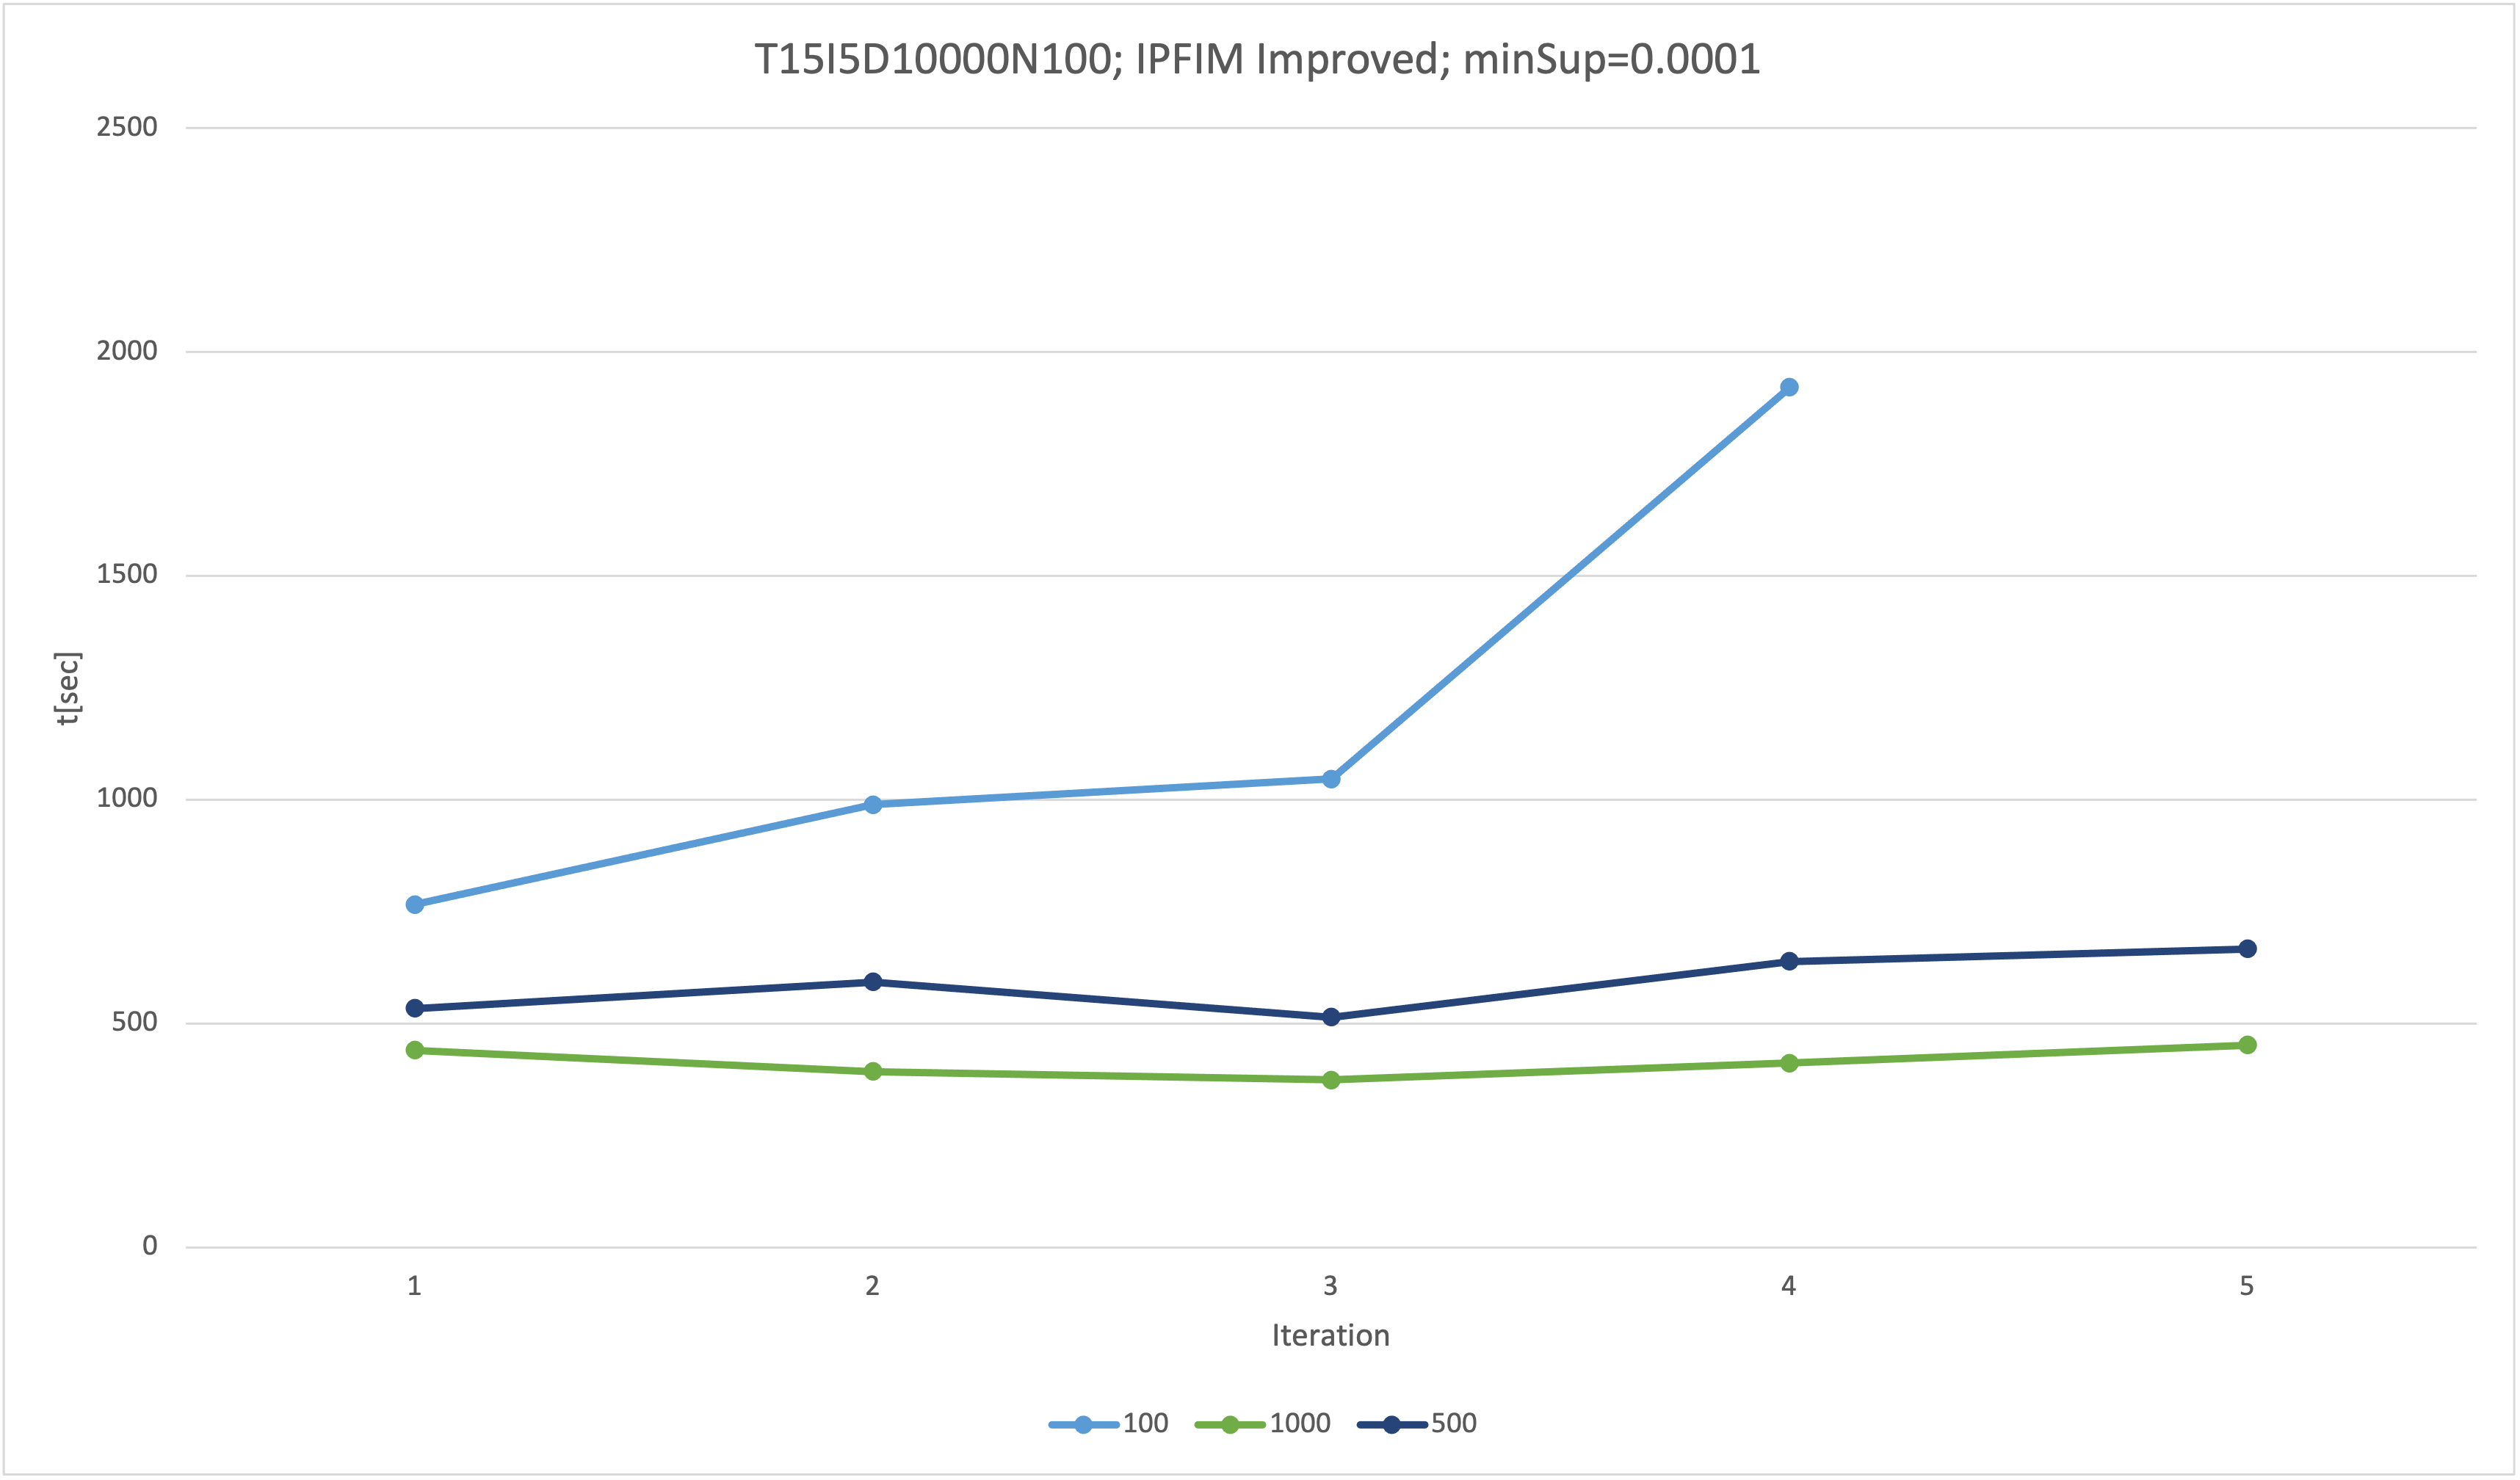
\includegraphics[width=\linewidth]{figures/4iterations/T15I5D10000N100_ipfim_imp_0001}
  \caption{T15I5D10000N100, minSup = 0.0001,  IPFIM Improved 100\textbar 1000\textbar 500 partitions}
  \label{fig:T15I5D10000N100_ipfim_imp_0001}
\end{figure}

\begin{figure}
  \centering
  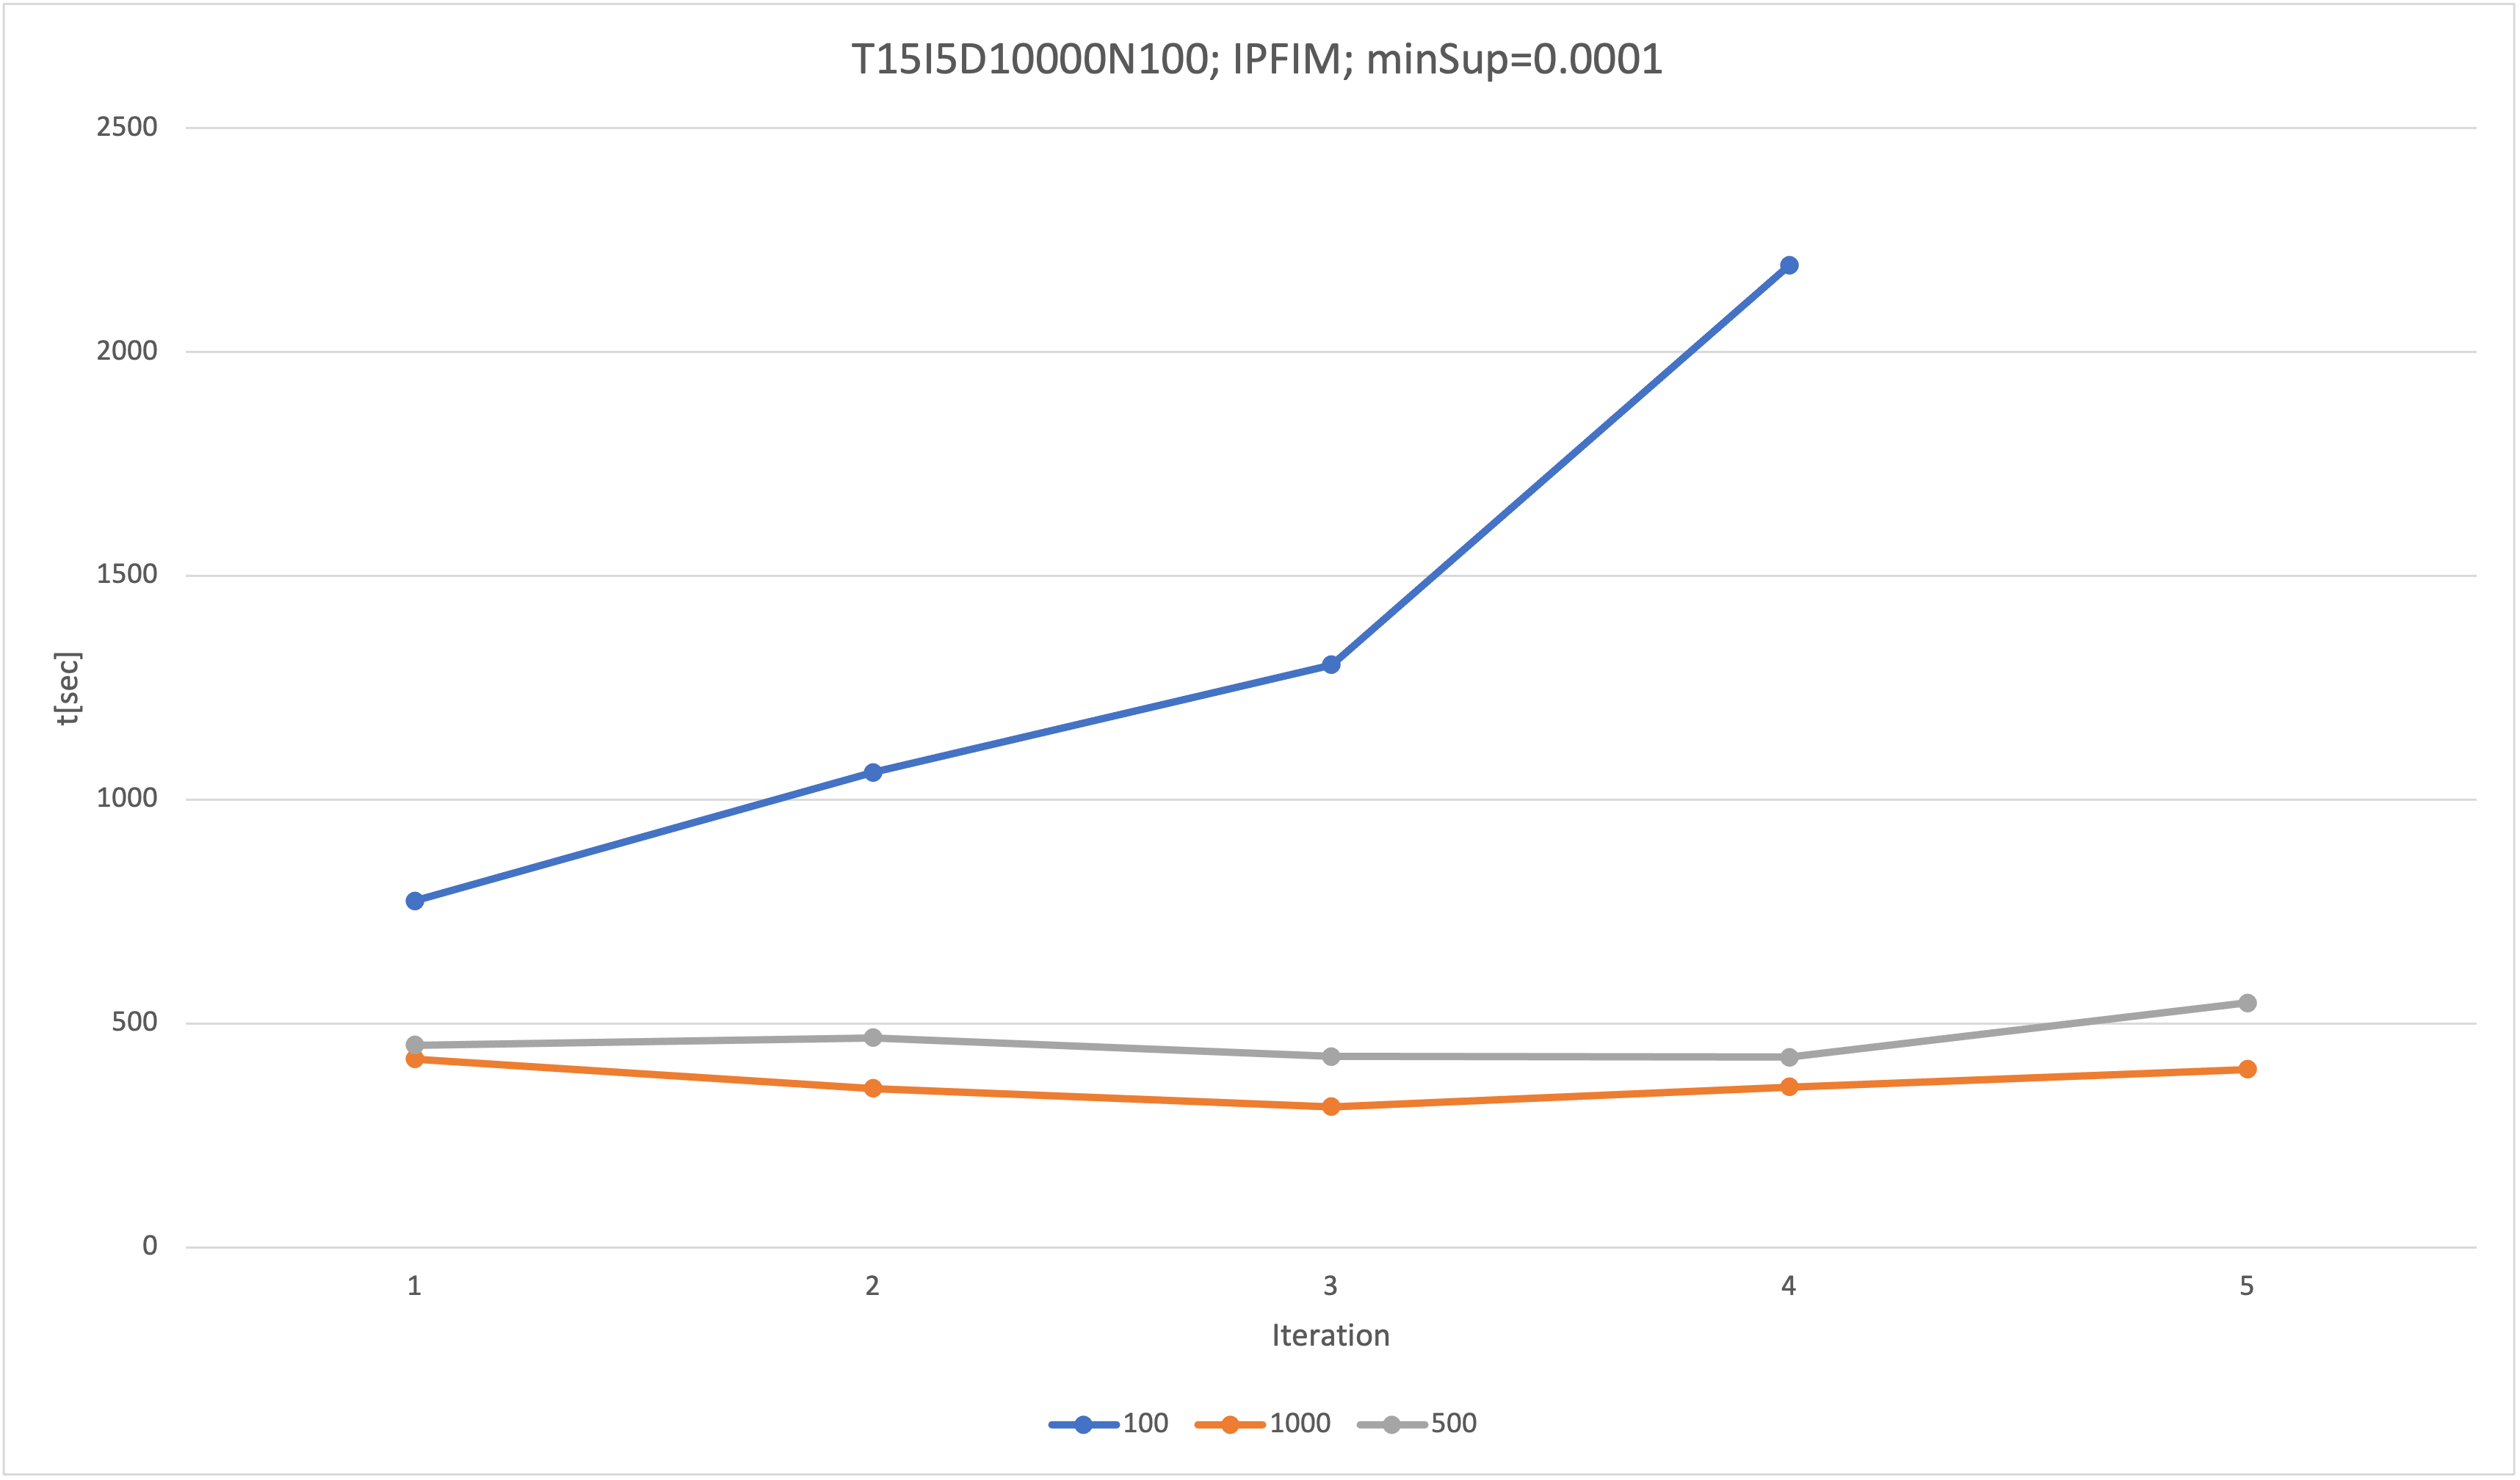
\includegraphics[width=\linewidth]{figures/4iterations/T15I5D10000N100_ipfim_0001}
  \caption{T15I5D10000N100, minSup = 0.0001,  IPFIM 100\textbar 1000\textbar 500 partitions}
  \label{fig:T15I5D10000N100_ipfim_0001}
\end{figure}

\begin{figure}
  \centering
  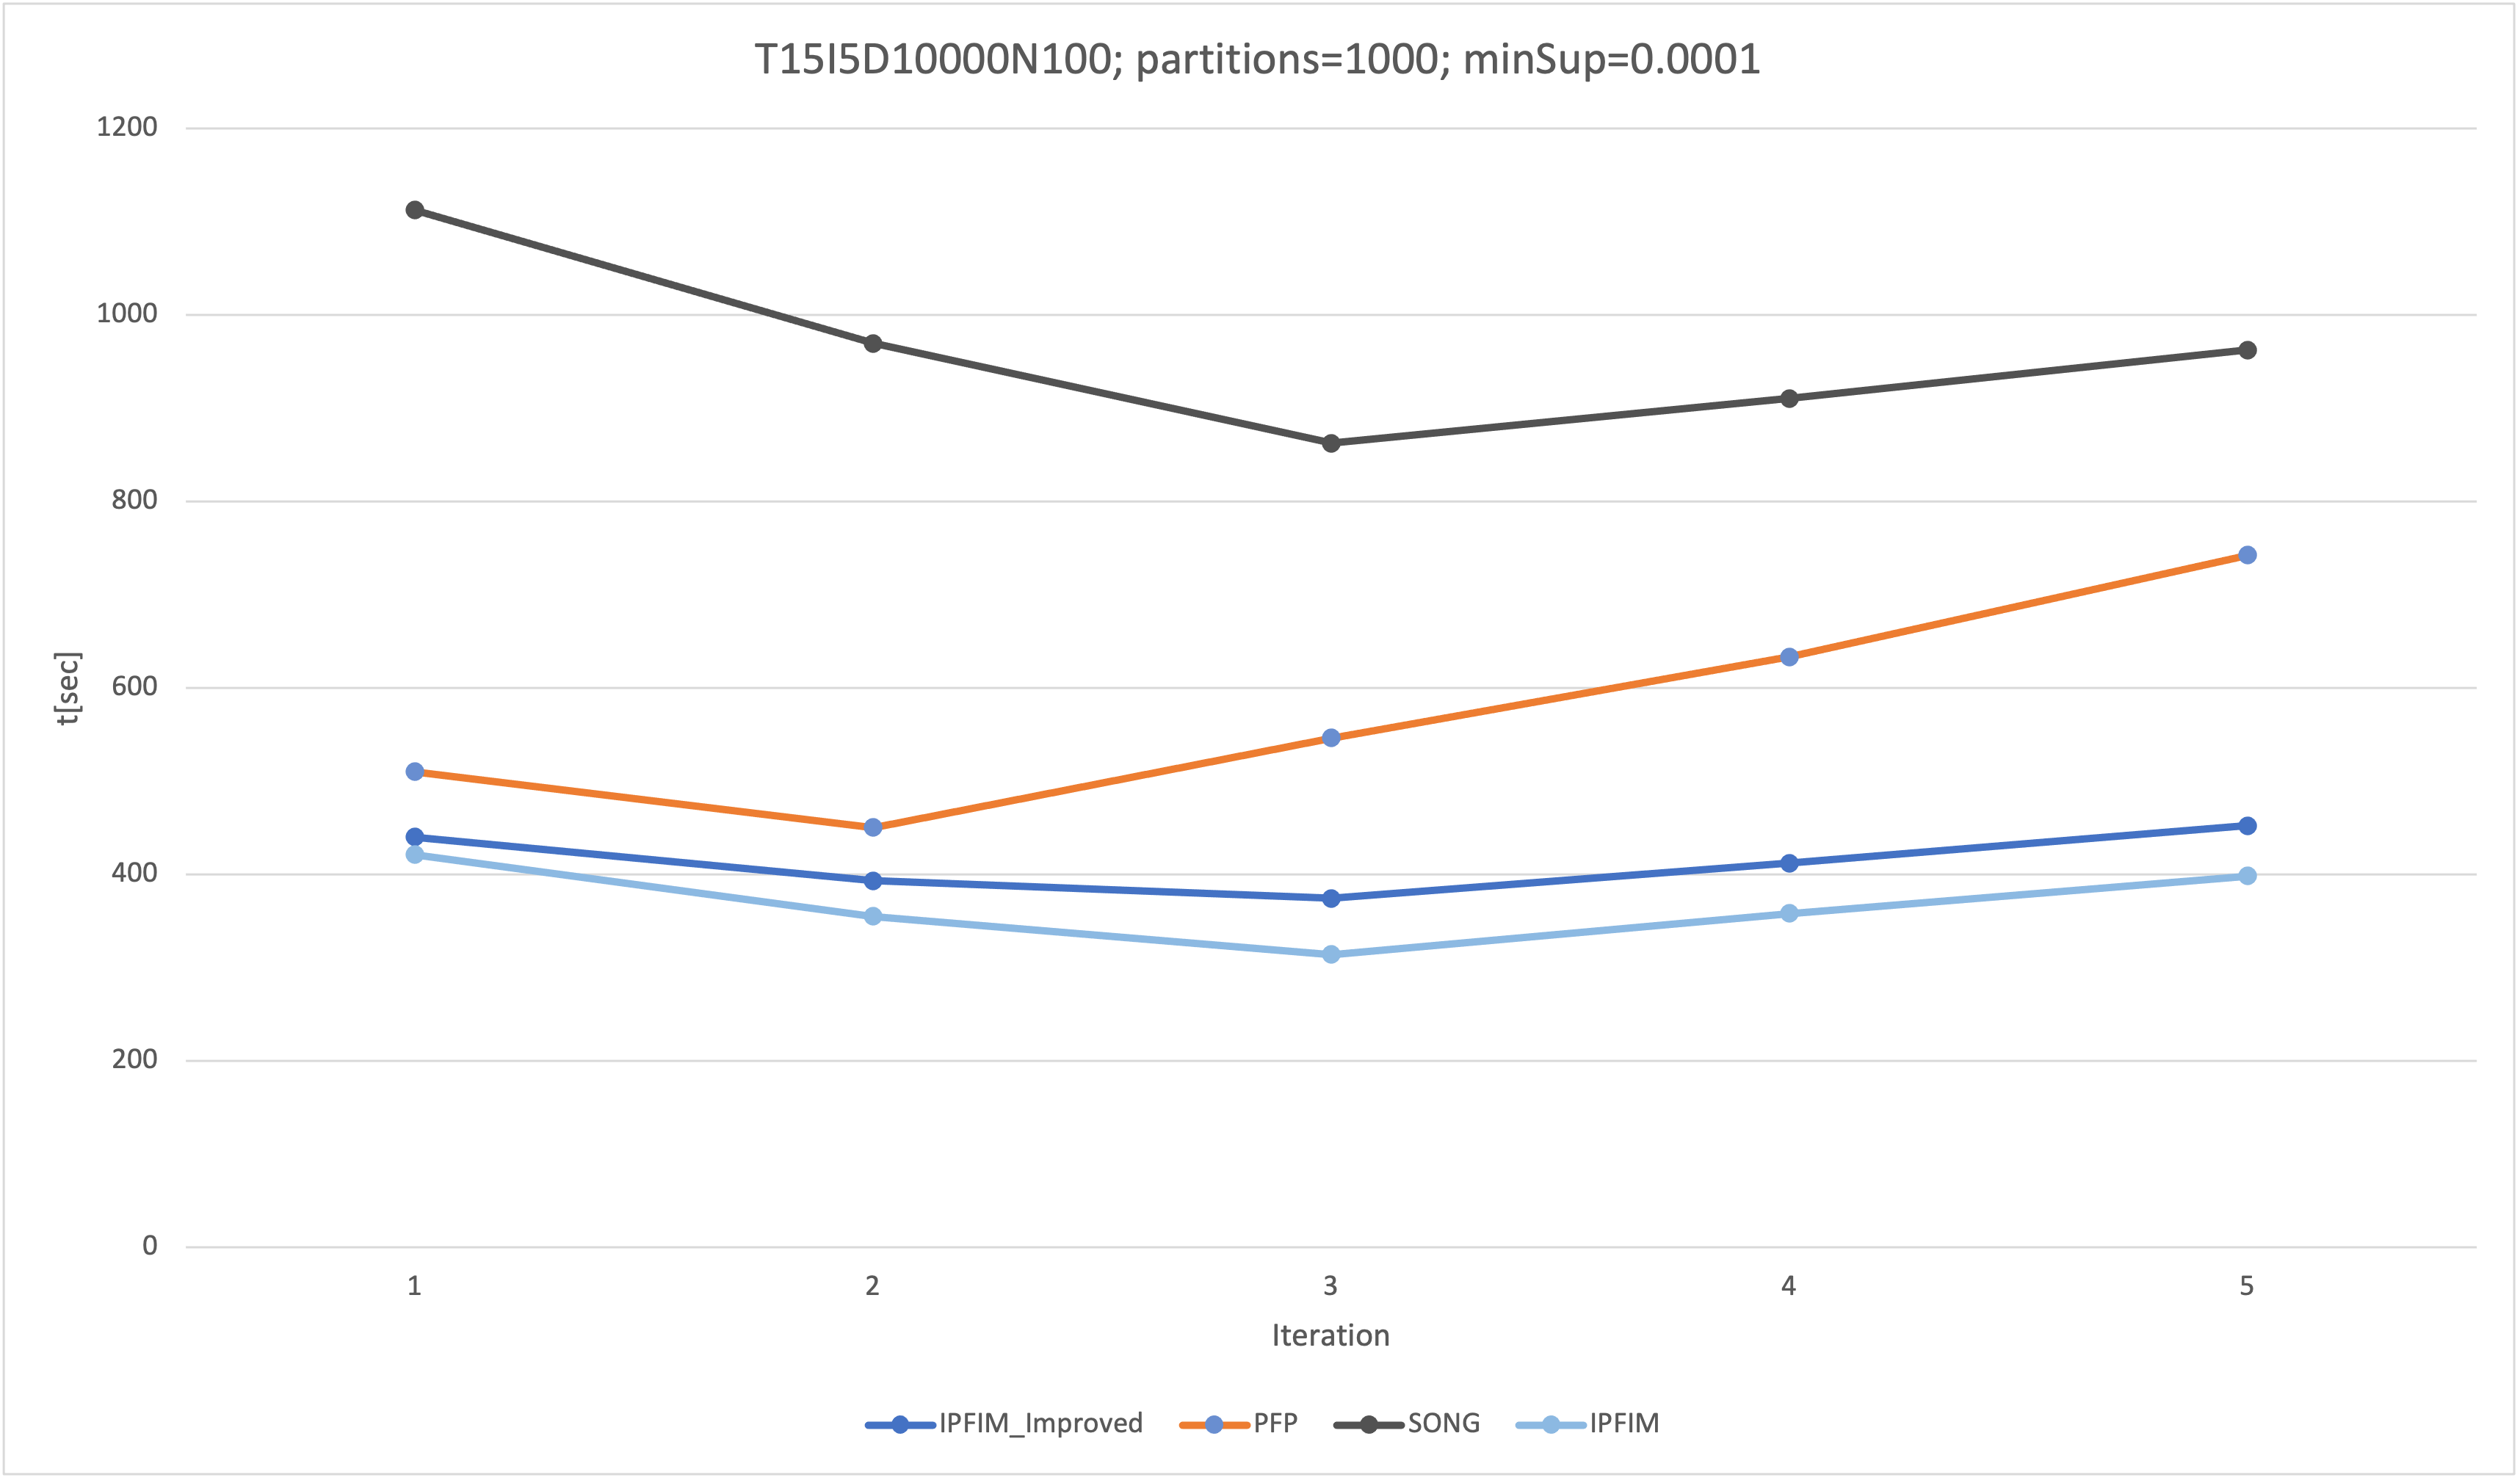
\includegraphics[width=\linewidth]{figures/4iterations/T15I5D10000N100_1000part_0001}
  \caption{T15I5D10000N100, minSup = 0.0001,  1000 partitions}
  \label{fig:T15I5D10000N100_1000part_0001}
\end{figure}

\begin{figure}
  \centering
  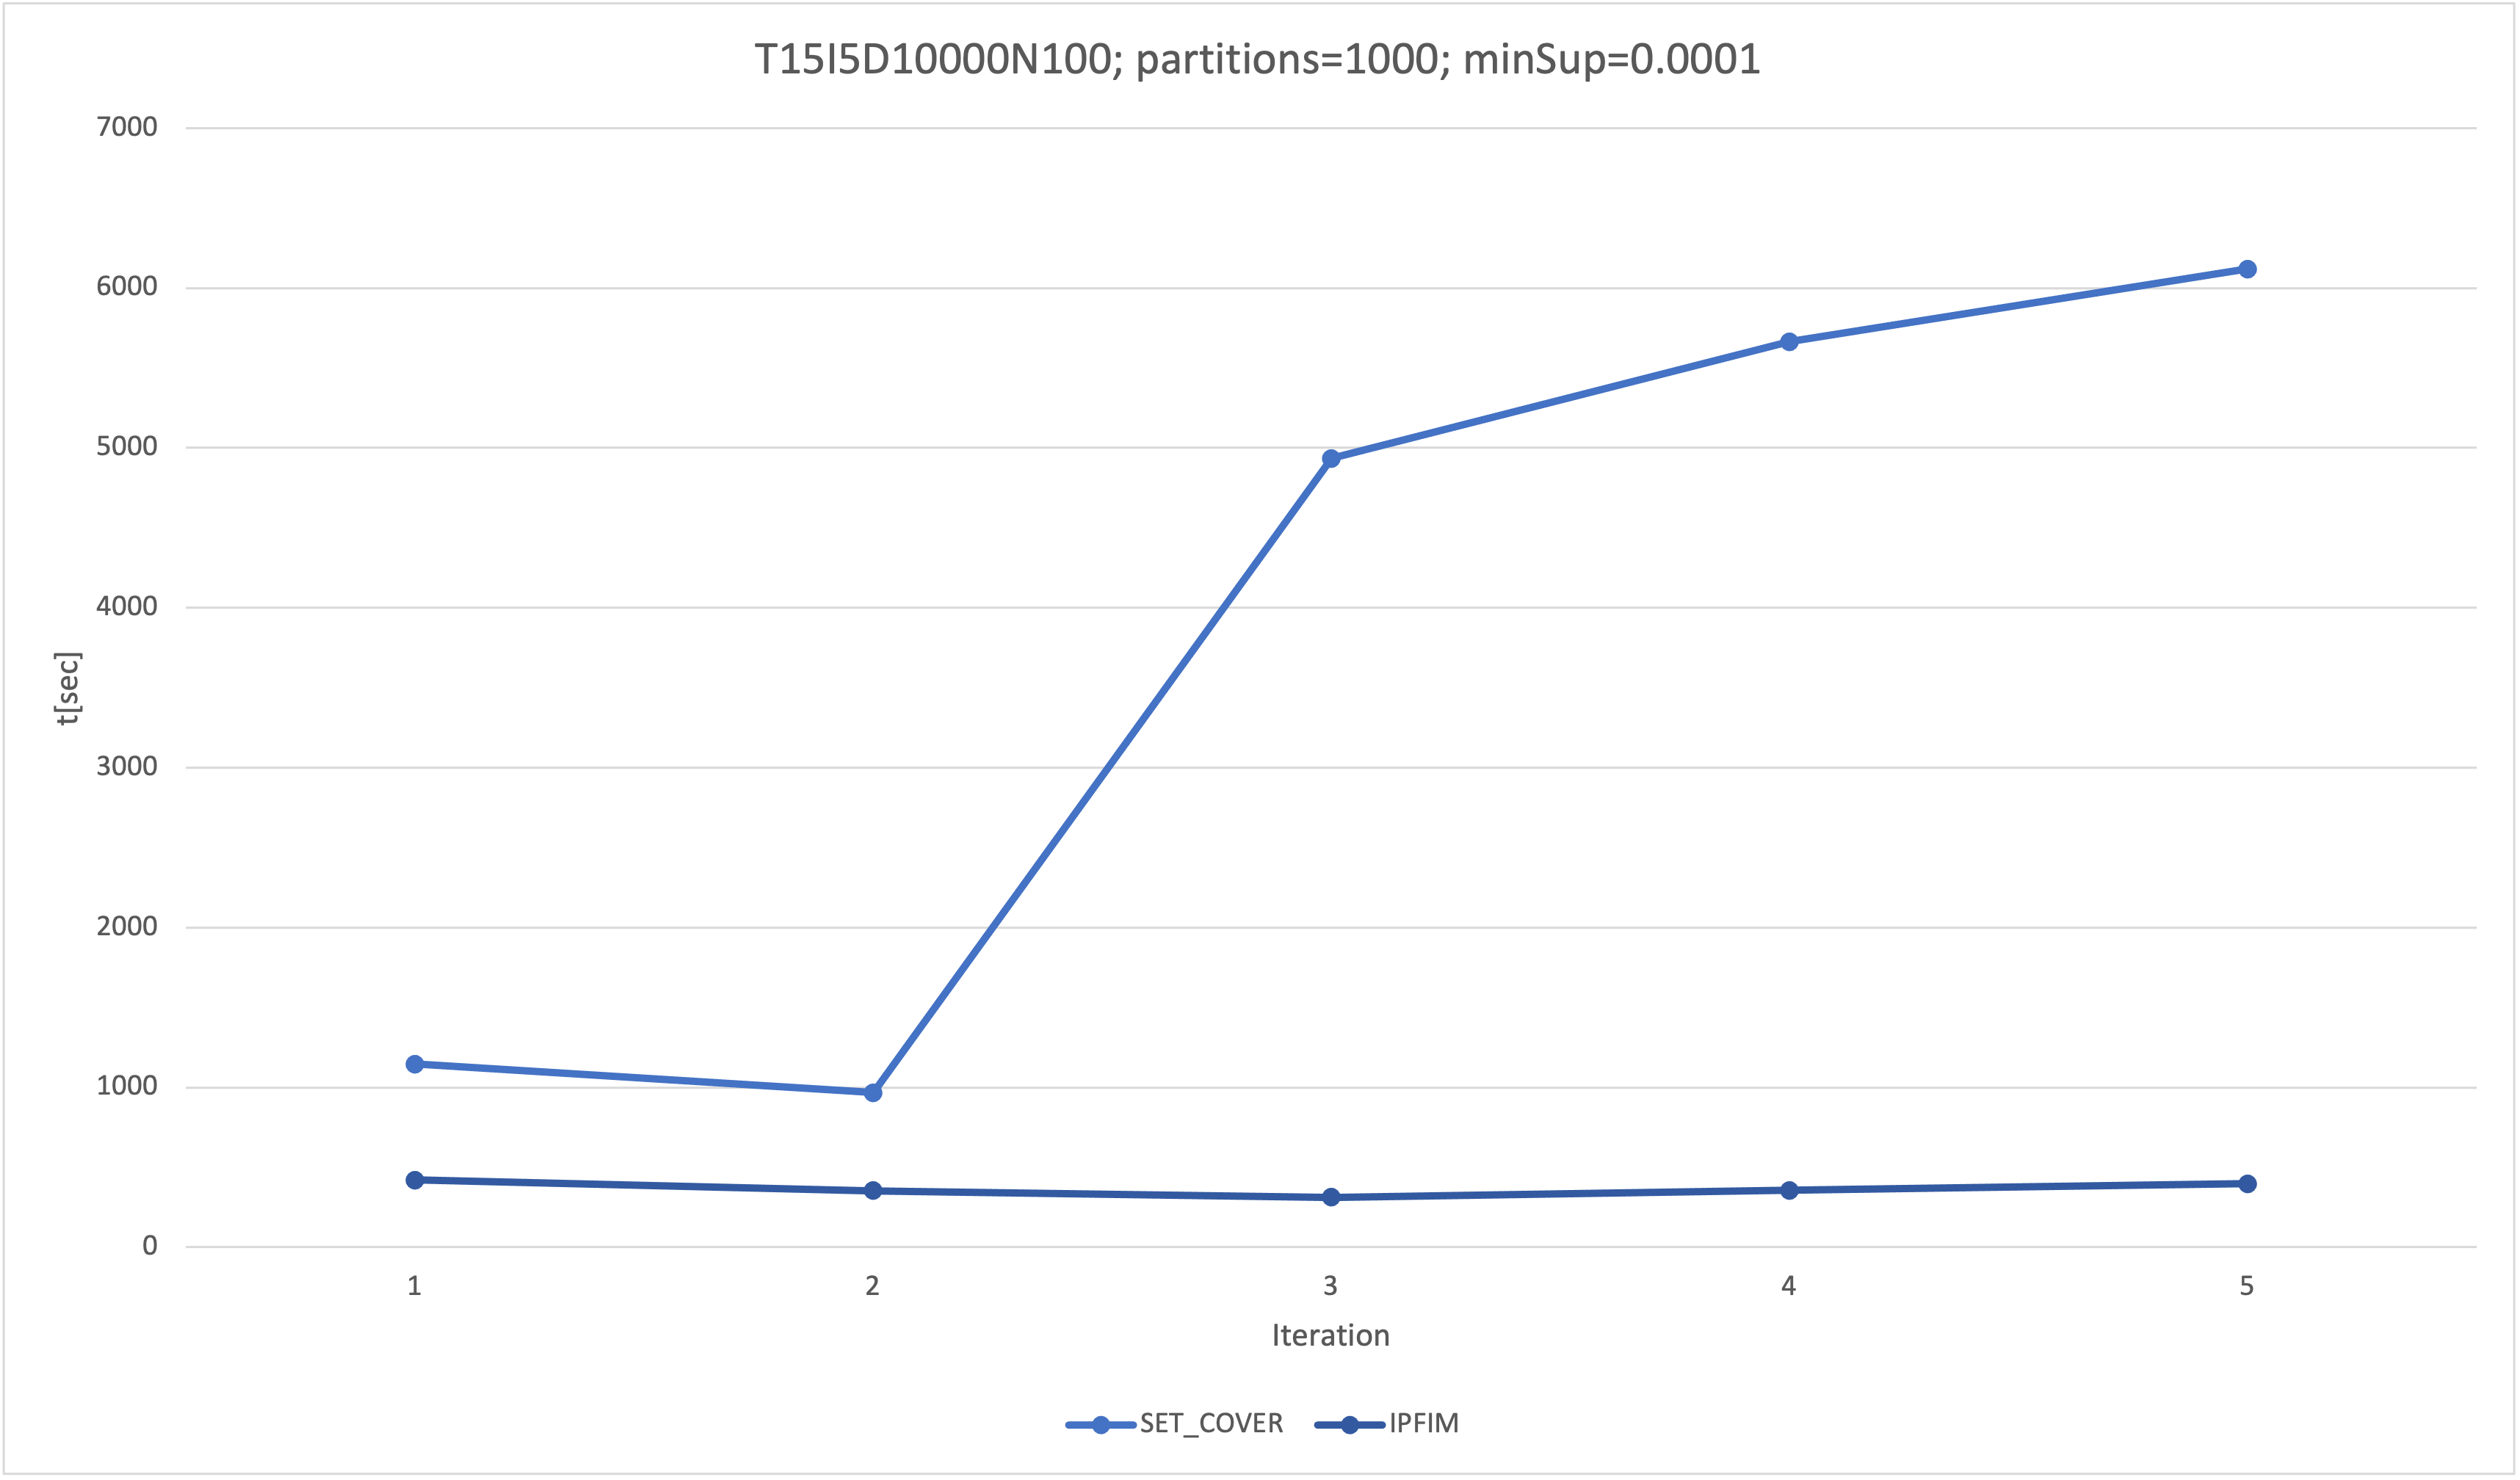
\includegraphics[width=\linewidth]{figures/4iterations/T15I5D10000N100_1000part_SETCOVER_0001}
  \caption{T15I5D10000N100, minSup = 0.0001,  1000 partitions, Set cover vs IPFIM}
  \label{fig:T15I5D10000N100_1000part_SETCOVER_0001}
\end{figure}



\begin{figure}
  \centering
  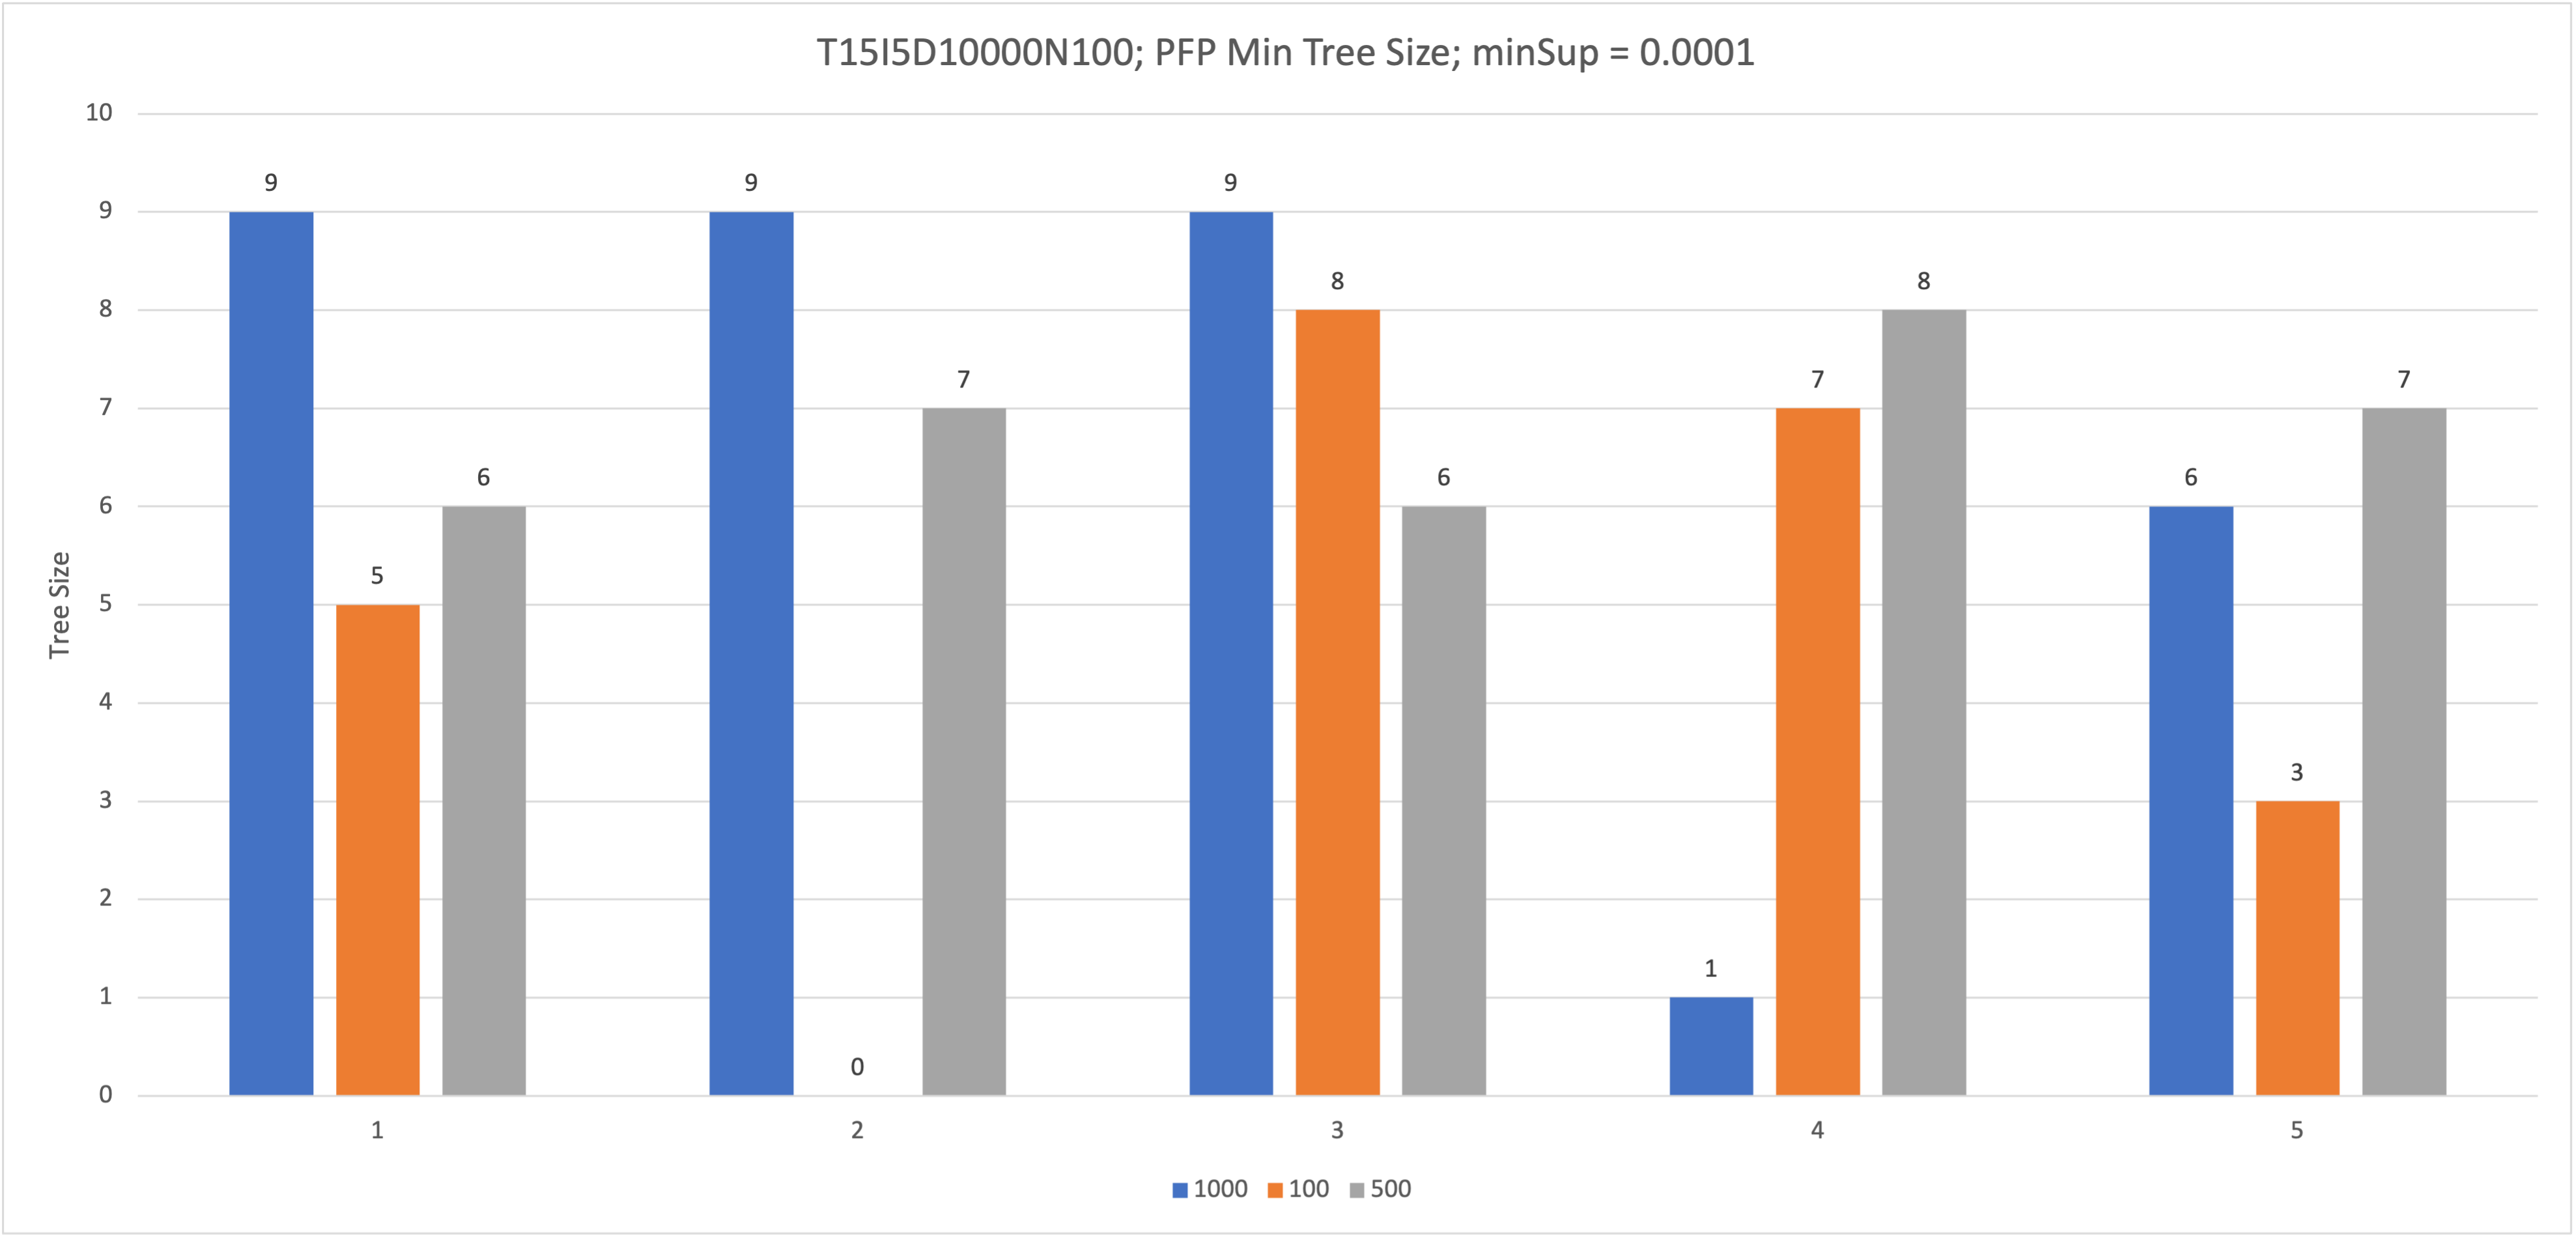
\includegraphics[width=\linewidth]{figures/4iterations/T15I5D10000N100_MinTree_PFP_0001}
  \caption{T15I5D10000N100, minSup = 0.0001,  PFP, Min Tree size for partitions}
  \label{fig:T15I5D10000N100_MinTree_PFP_0001}
\end{figure}

\begin{figure}
  \centering
  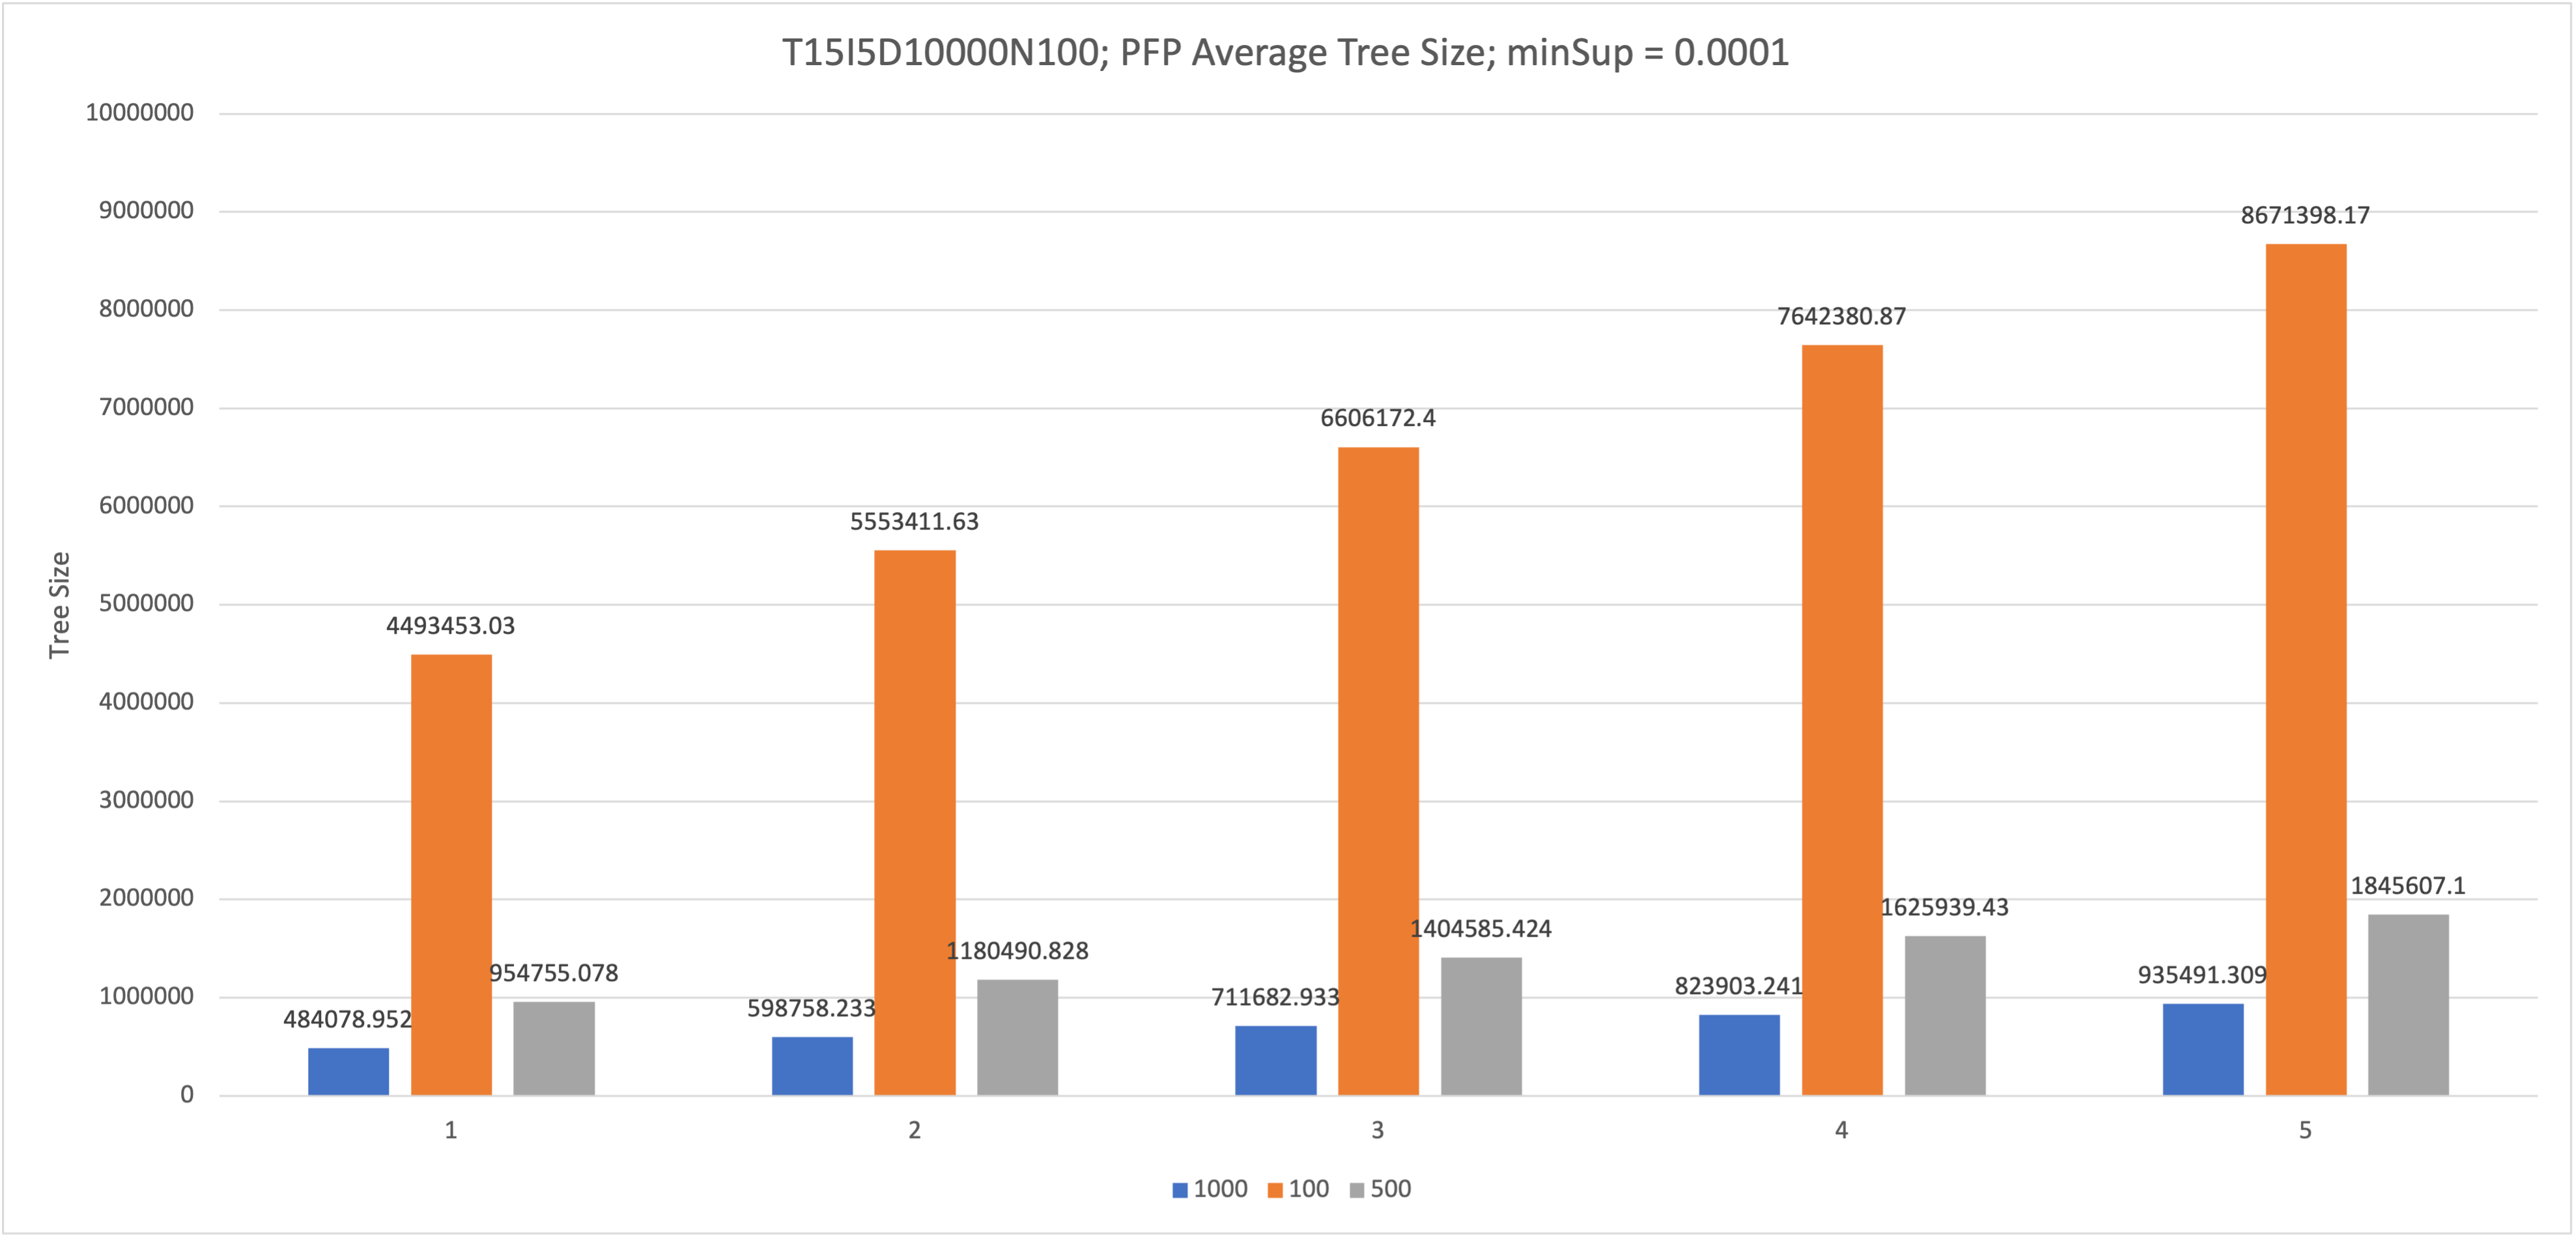
\includegraphics[width=\linewidth]{figures/4iterations/T15I5D10000N100_AvgTree_PFP_0001}
  \caption{T15I5D10000N100, minSup = 0.0001,  PFP, Average Tree size for partitions}
  \label{fig:T15I5D10000N100_AvgTree_PFP_0001}
\end{figure}

\begin{figure}
  \centering
  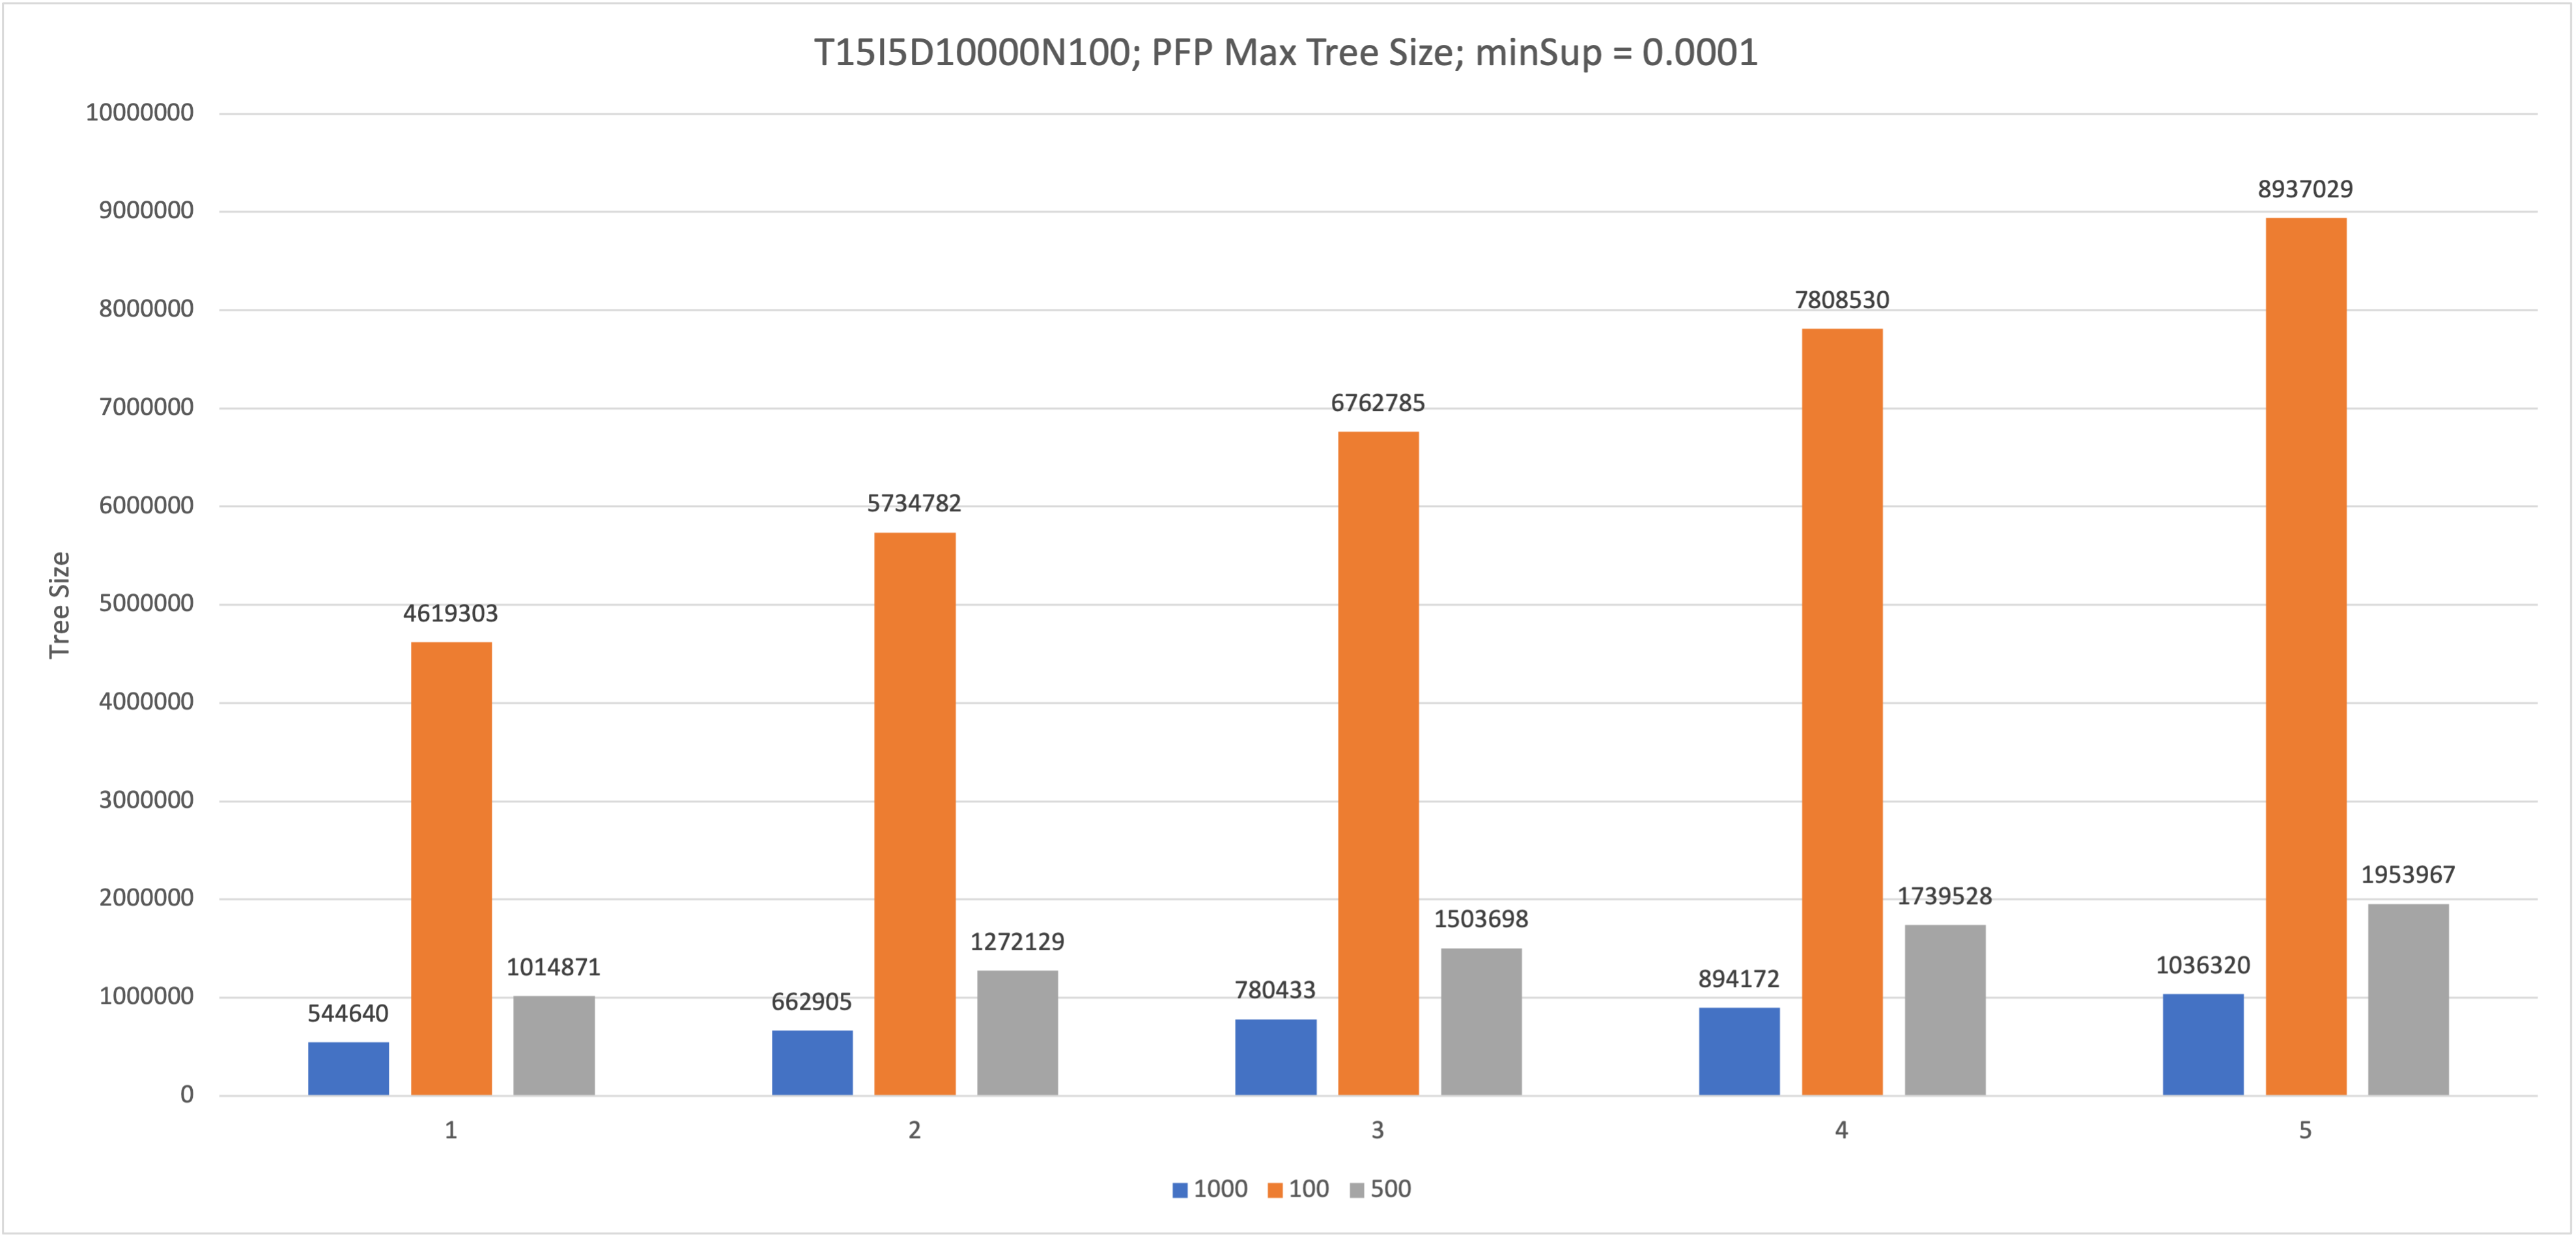
\includegraphics[width=\linewidth]{figures/4iterations/T15I5D10000N100_MaxTree_PFP_0001}
  \caption{T15I5D10000N100, minSup = 0.0001,  PFP, Maximum Tree size for partitions}
  \label{fig:T15I5D10000N100_MaxTree_PFP_0001}
\end{figure}

\begin{figure}
  \centering
  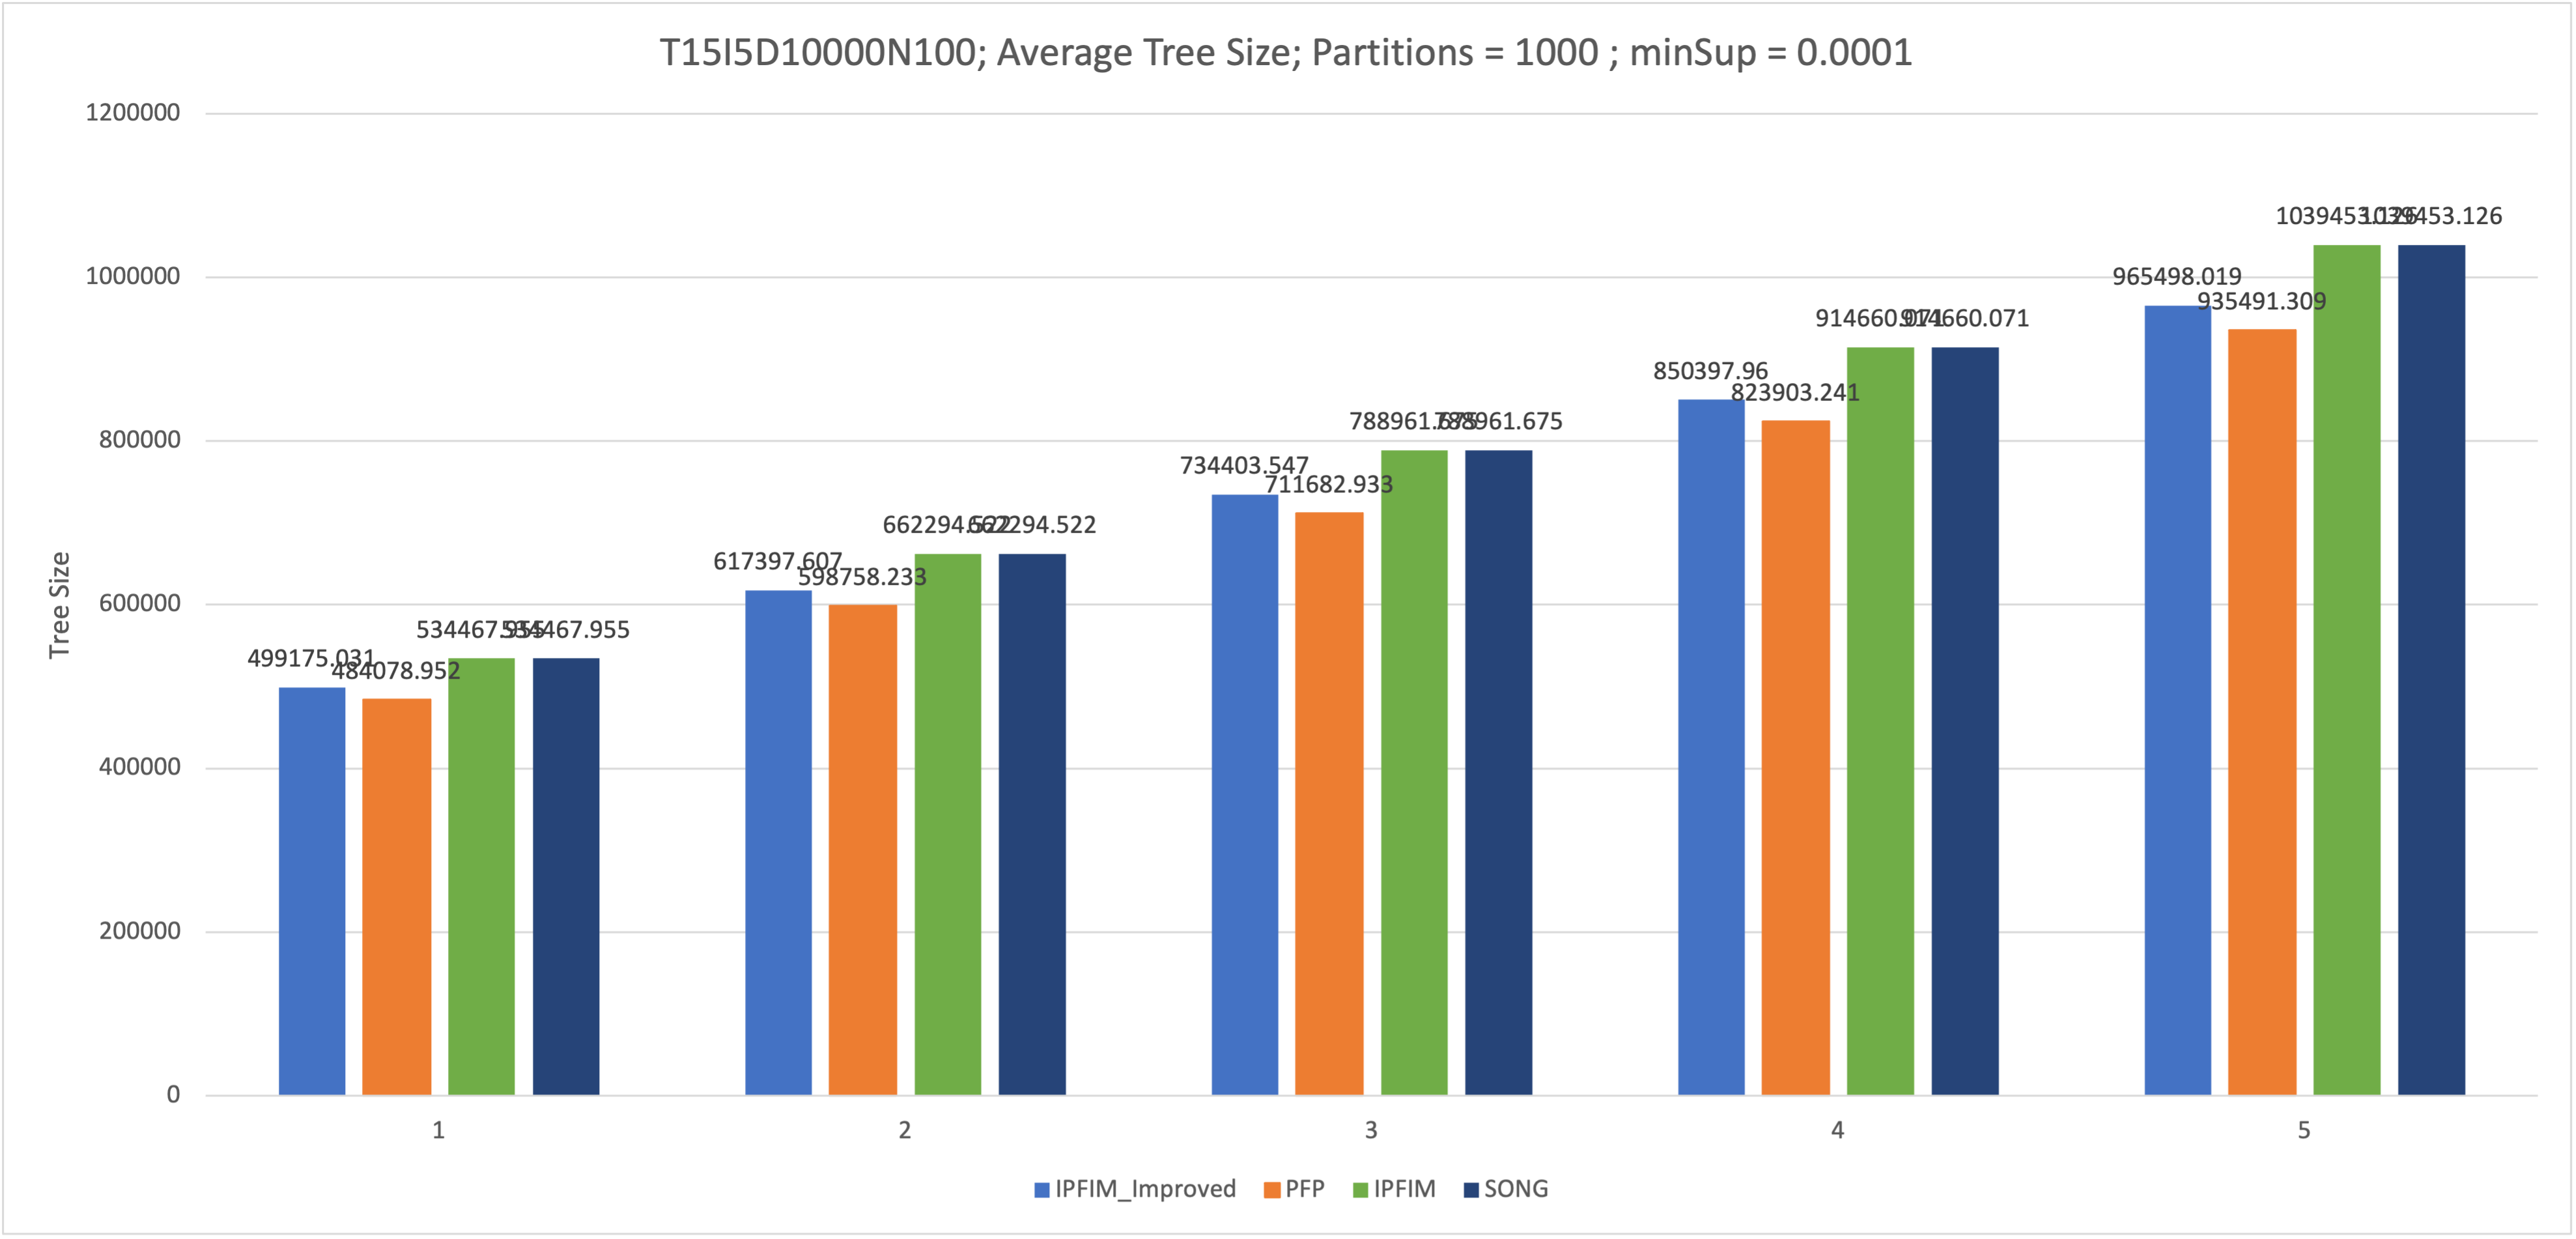
\includegraphics[width=\linewidth]{figures/4iterations/T15I5D10000N100_AvgTree_Partitins1000_0001}
  \caption{T15I5D10000N100, minSup = 0.0001,  Average Tree size for 1000 partitions}
  \label{fig:T15I5D10000N100_AvgTree_Partitins1000_0001}
\end{figure}



\begin{figure}
  \centering
  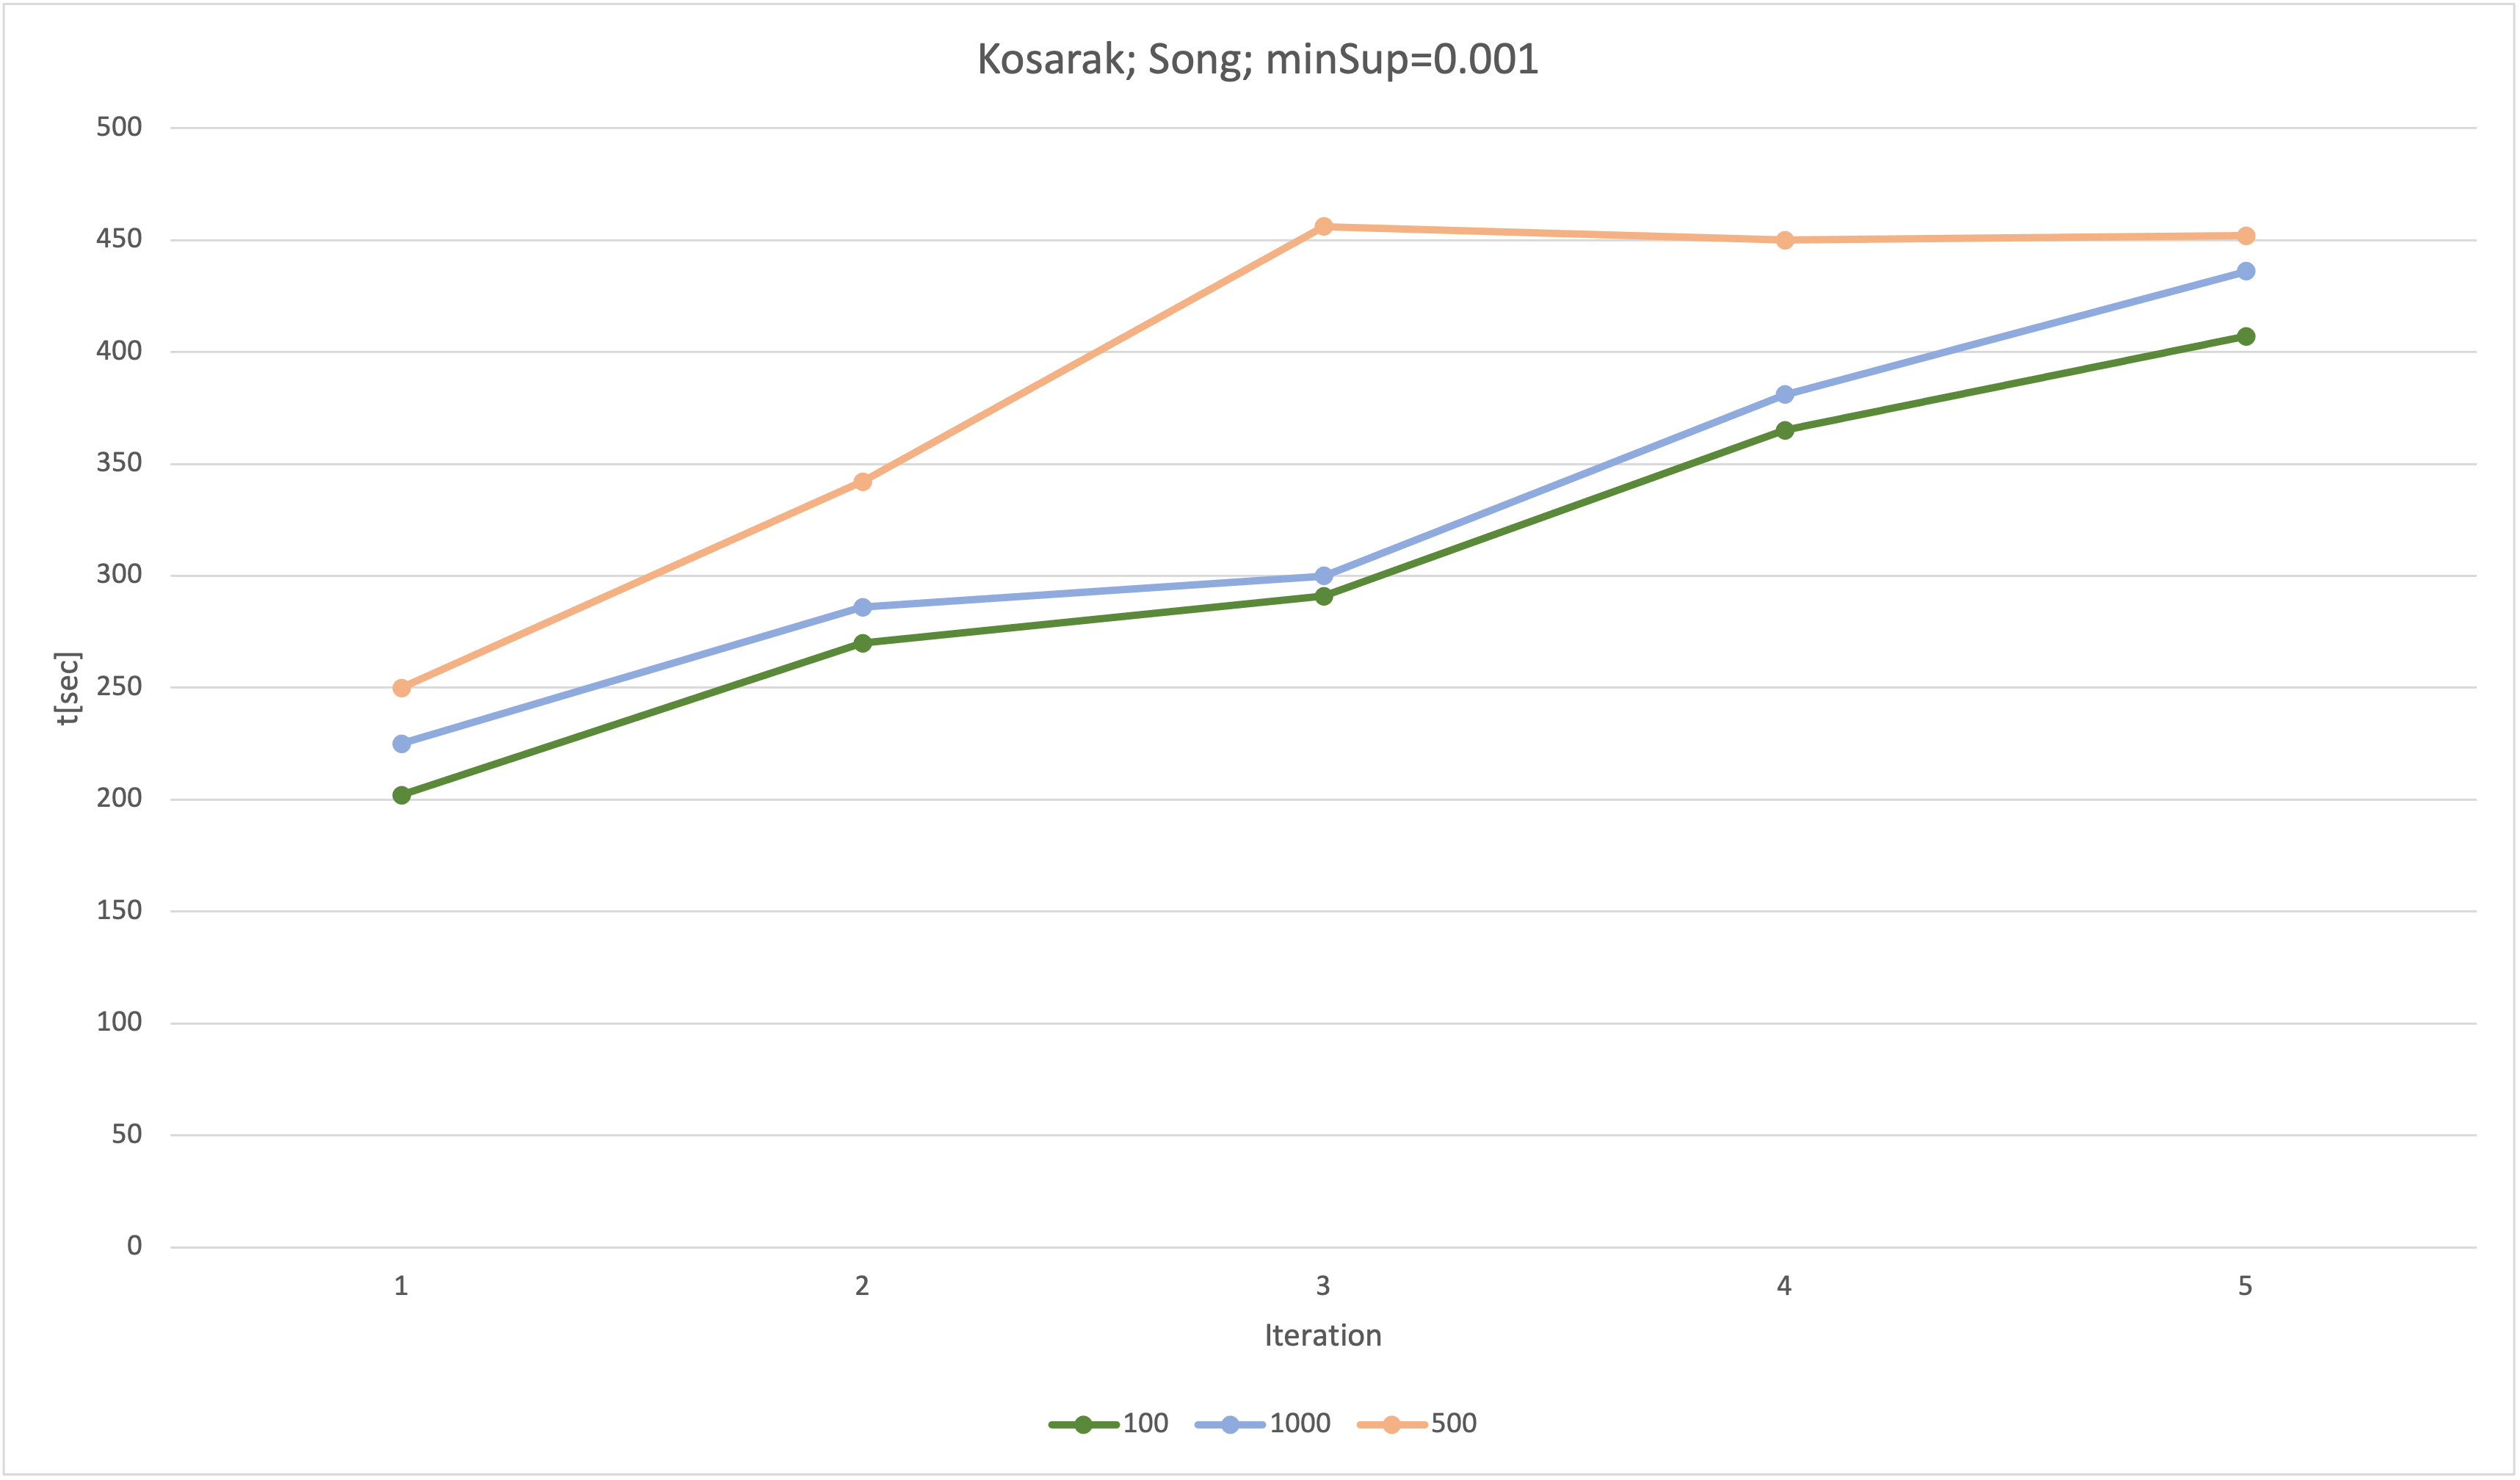
\includegraphics[width=\linewidth]{figures/4iterations/kosarak_song_001}
  \caption{kosarak, minSup = 0.001, SONG 100\textbar 1000\textbar 500 partitions}
  \label{fig:kosarak_song_001}
\end{figure}

%
%\begin{figure}[h!]
%  \centering
%  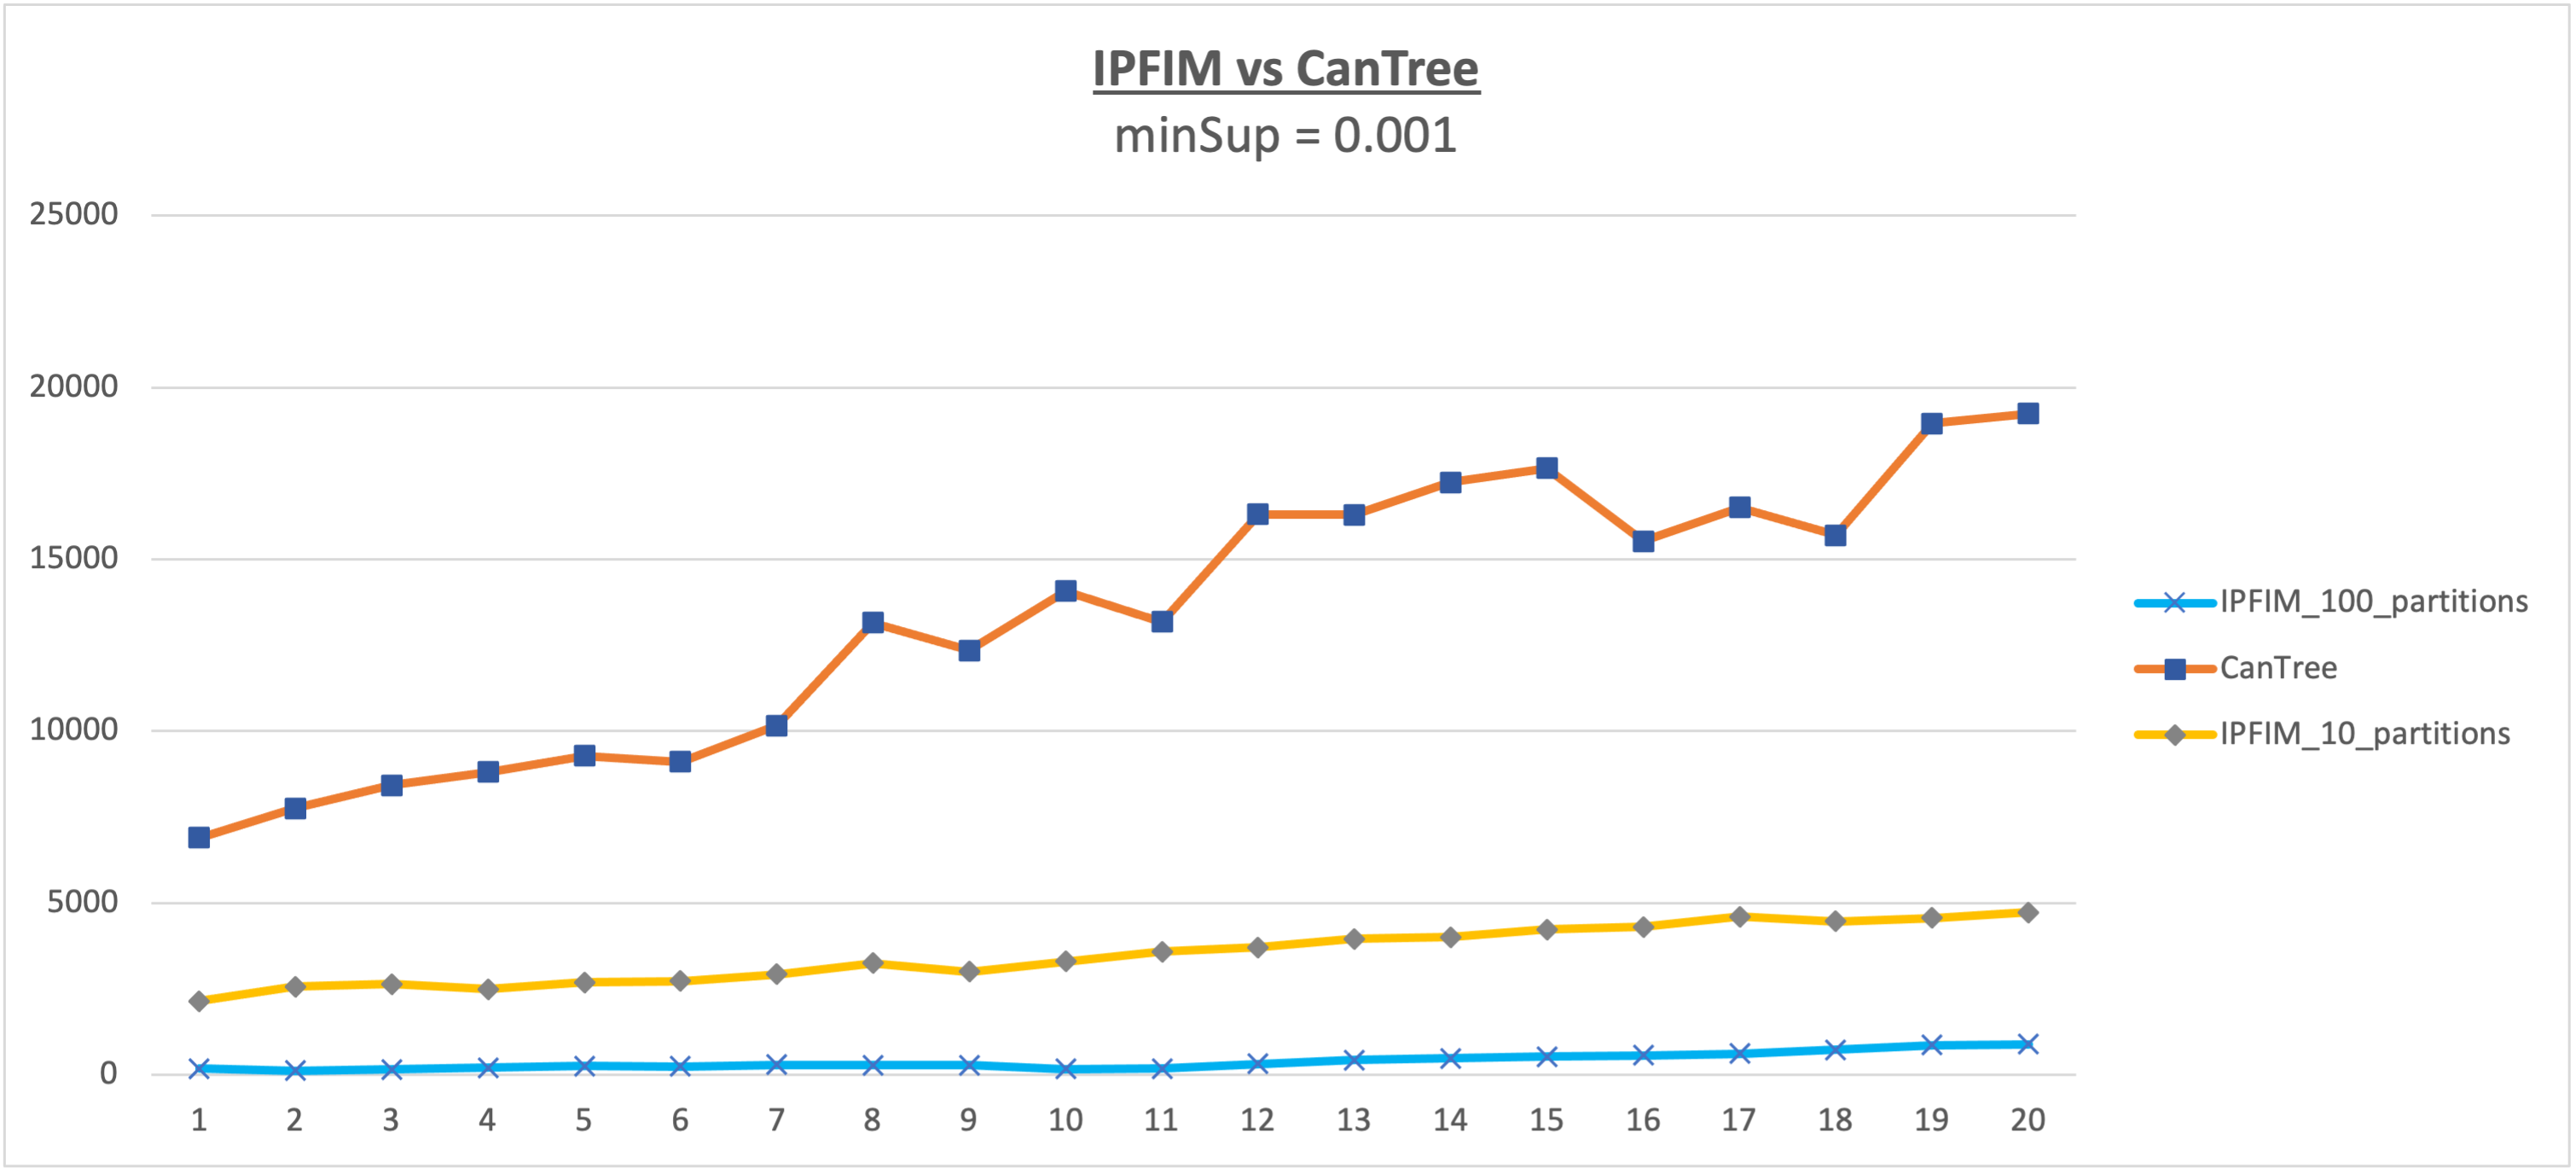
\includegraphics[width=\linewidth]{figures/IPFIM_VS_CANTREE_001_KOS}
%  \caption{IPFIM vs CanTree Kosarak}
%  \label{fig:IPFP1M0001_10_100}
%\end{figure}


\subsection{IPFIM vs PFP}
 For correct PFP~\cite{li2008pfp} mining, a read of all the dataset till that point needs to be performed.
\subsubsection{Synthetic Dataset}
A comparison for 10M transactions (T15D10MN100K) with minSupport of 0.001, 1K partitions is seen at \autoref{fig:PFPvsIPFP}.

\subsubsection{Kosarak Dataset}
A comparison with minSupport of 0.001, partitions of 10 and 100 is seen at \autoref{fig:PFPvsIPFPKos}.


%%\begin{figure}
%%  \centering
%%  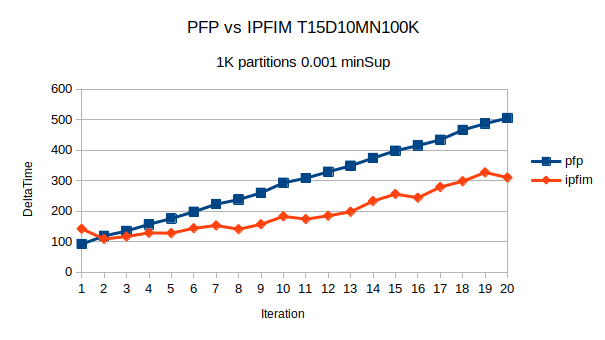
\includegraphics[width=\linewidth]{figures/PFPvsIPFIM0_001_10M}
%%  \caption{PFP vs IPFIM 10M}
%%  \label{fig:PFPvsIPFP}
%%\end{figure}
%
%\begin{figure}
%  \centering
%  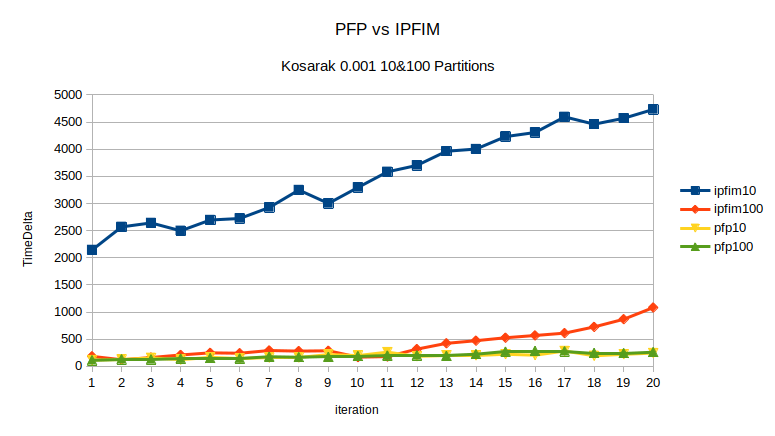
\includegraphics[width=\linewidth]{figures/PFPvsIPFIM0_001_Kosarak}
%  \caption{PFP vs IPFIM Kosarak}
%  \label{fig:PFPvsIPFPKos}
%\end{figure}

%\begin{figure}[h!]
%  \centering
%  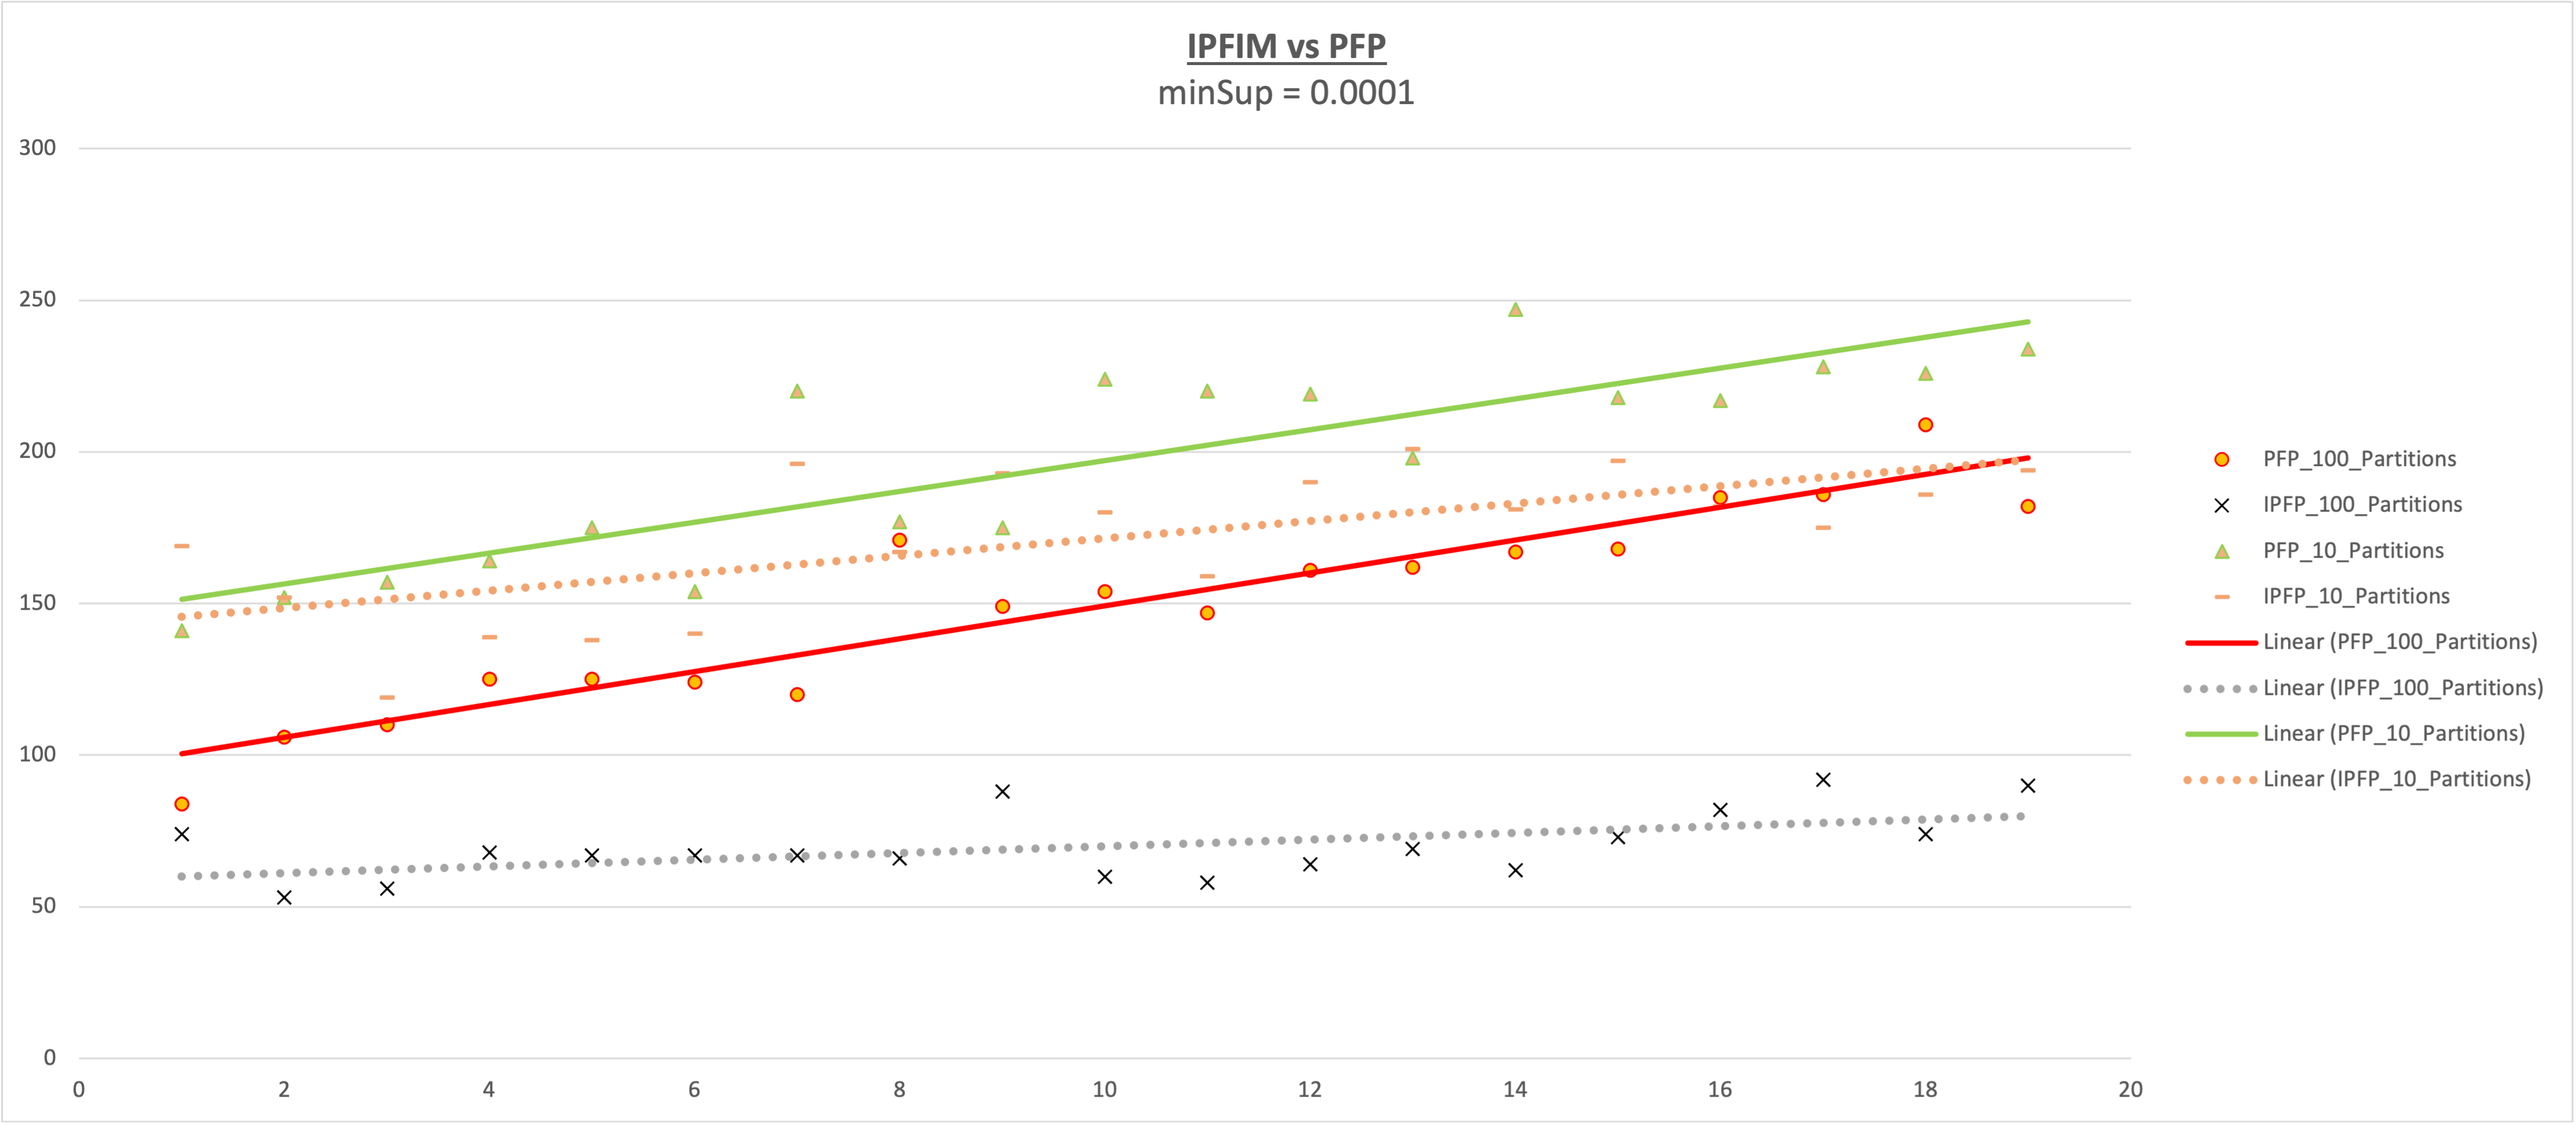
\includegraphics[width=\linewidth]{figures/IPFIM_VS_PFP_0001_T15D1M10K}
%  \caption{IPFIM vs PFP 0.0001 T15D1M10K}
%  \label{fig:IPFP_vs_PFP_0001_T15D1M10K}
%\end{figure}

\subsection{improved-IPFIM vs PFP}
\subsection{improved-IPFIM vs Song et al.}
\subsection{set-cover-IPFIM vs Song et al.}